% importa variabili globali
% definizione variabili globali
\def\GRUPPO {\textit{DazzleWorks}}

\def\PROGETTO {\textbf{Premi}}

\def\COMMITTENTE {Prof. Vardanega Tullio, \\ & Dr. Cardin Riccardo}

\def\EMAIL {dazzleworksgroup@gmail.com}

\def\LOGO {../../template/img/logo.png}

\def\INTESTAZIONE {../../template/img/intestazione.png}
\def\PIEDIPAGINA {../../template/img/piedipagina.png}

\def\G {{\small $_G$}}



% definizione variabili locali
\def\DOCUMENTO{Definizione di Prodotto}
\def\VERSIONE{3.0.0}

\def\DESCRIZIONE{Documento che definisce in dettaglio l'architettura del prodotto \PROGETTO.}

\def\REDATTORE {Burlin Valerio \\ & Suierica Bogdan \\ & Ros Fabio}
\def\VERIFICATORE {Carraro Nicola}
\def\RESPONSABILE {Agostinetto Matteo}

\def\USO {Esterno}

\def\DISTRIBUZIONE {\GRUPPO{}\\ & \COMMITTENTE{}\\ & \PROPONENTE{}\\}

\def\DESCRIZIONE {Documento che definisce in dettaglio l'architettura del prodotto \PROGETTO.}

\def\SCOPE {\textit{\$scope}}


% abilita (true) / disabilita (false) indice, lista tabelle, lista figure
\def\INDICE	{true}
\def\TABELLE {true}
\def\FIGURE {true}


% importa struttura
\documentclass[a4paper]{article}

% ----- definizioni -----
\def\TITLE		{\mbox{\GRUPPO}}
\def\SUBTITLE	{\SIGLA, \PROGETTO}


% ----- nuovi comandi -----
% fornisce il caption per riferirsi ad una particolare sezione
\newcommand{\numref}[1]{\textsf{\textsl{``\nameref{#1}'' (\ref{#1})}}}


% ----- package -----
\usepackage[T1]{fontenc}   % codifica dei font in uscita
\usepackage[utf8x]{inputenc}   % lettere accentate da tastiera
\usepackage[italian]{babel}   % lingua principale del documento
\usepackage[a4paper, top= 3cm, bottom= 3cm, left= 3cm, right= 3cm, bindingoffset= 5mm]{geometry} % impostazione margini

\usepackage{amssymb} %

\usepackage{booktabs} % comandi aggiuntivi per le tabelle

\usepackage{calc} % espressioni aritmetiche
\usepackage{caption} % descrizione figure, ecc
\usepackage{chapterbib} % inclusione delle bibliografie

\usepackage{datatool} % manipolazione dati
\usepackage{dcolumn} % array in tabular

\usepackage{epstopdf} % conversione eps--> pdf
\usepackage{enumitem} % personalizzazione liste
\usepackage{eurosym} % simbolo euro

\usepackage{fancyhdr}   %personalizzazione dello stile
\usepackage{float} % definizione di oggetti floating (es. figure, tabelle)
\usepackage[bottom]{footmisc} % personalizzazione note

\usepackage[toc]{glossaries}	% glossario
\usepackage{graphicx, subfigure} % pacchetto grafica testo
\usepackage{grffile} % estende gestione filename graphic

\usepackage[colorlinks=true, urlcolor=blue, citecolor=black, linkcolor=black, hyperindex, breaklinks]{hyperref} % gestione dei link

\usepackage{ifthen}	% costrutto ifthenelse

% \usepackage{listings} % inserimento pezzi di codice
\usepackage{longtable} % tabelle su più pagine

\usepackage{pgf} % grafica postscript e PDF
\usepackage{pgfplots}	% composizione di grafici
\pgfplotsset{/pgf/number format/use comma, compat=newest}	% opzioni per i grafici

\usepackage{multirow} % span multiriga

\usepackage{tabularx, array} % crea paragrafi a colonne
\usepackage{titlesec} % personalizzazione titoli
\usepackage{tikz} % gestione delle formule
\usepackage{totpages} % conta numero pagine

\usepackage{soul} % gestione letterspacing
\usepackage{subfigure} % gestione delle sottofigure

\usepackage{verbatim} % inserimento testo verbatim, non interpretato

\usepackage{wallpaper} % gestione background

\usepackage{xspace} % spazi automatici per le macro


% ----- posizione etichette -----
\captionsetup{tableposition=top, figureposition=bottom, font=small}


% ----- glossario -----
\loadglsentries{../../glossario/glossario.tex}
\renewcommand*{\glssymbolsgroupname}{Simboli}


% ----- stile pagina -----
\pagestyle{fancy}

	% header
	\fancypagestyle {firststyle} {	% definizione stile "firststyle"
		\fancyhf{}
	}

	% indentazione paragrafo
	%\setlength{\parindent} {0pt}
	\setlength{\headheight} {25pt}

	% intestazione
	\lhead{}
	\rhead{\nouppercase{\leftmark}}
	\renewcommand{\headrulewidth}{0pt}  % no linea sotto intestazione

	% piè di pagina
	\lfoot{\footnotesize{{\DOCUMENTO} \\ {\VERSIONE}}}
	\cfoot{}
	\rfoot{\thepage}
	\renewcommand{\footrulewidth}{0pt}   % no linea sopra piè di pagina


% ----- inizio documento -----
% ----- prima pagina -----
\begin{document}
\thispagestyle{firststyle}

\begin{center}

%   \vspace{7cm}
	\textbf{{\fontsize{40pt}{41pt}\selectfont \PROGETTO}} \\
	\rule{8cm}{3pt}
   
   \vspace{4cm}
   \includegraphics[height= 4cm] {\LOGO}
   
	\vspace{1cm}
   {\fontsize{30pt}{31pt}\selectfont \textbf{\GRUPPO}}
	
	\vspace{5cm}
	{\fontsize{18pt}{24pt}\selectfont \textbf{\DOCUMENTO}}
	
%	\vspace{1cm}
	\begin{center}
		\begin{tabular}{r|l}
				\textbf{Versione} & \VERSIONE \\
				\textbf{Redattori} & \REDATTORE \\
				\textbf{Verificatori} & \VERIFICATORE \\
				\textbf{Responsabili} & \RESPONSABILE \\
				\textbf{Uso} & \USO \\
				\textbf{Lista di distribuzione} & \DISTRIBUZIONE
		\end{tabular}
	\end{center}

	\vspace{1cm}
	\textbf{\DESCRIZIONE}

\end{center}


\newpage

% ----- pagine successive -----
\ULCornerWallPaper{1}{\INTESTAZIONE}
\LLCornerWallPaper{1}{\PIEDIPAGINA}

%\thispagestyle{empty}

\newpage

% diario delle modifiche


% numerazione pagine indici
\pagenumbering{Roman}


% registro delle modifiche
\newpage
\section*{Registro delle modifiche}

\begin{table}[h]
\centering
\begin{tabular}{|c|p{0.3\textwidth}|c|c|c|}
	\toprule
		\textbf{Versione} & \textbf{Modifiche} & \textbf{Autore} & \textbf{Ruolo} & \textbf{Data}\\
	\midrule
	\midrule
		v1.0.0 & \textit{Approvazione documento} & Suierica Bogdan & \textit{Responsabile di Progetto} & 2015-06-23\\
	\midrule
		v0.1.0 & \textit{Verifica documento} & Agostinetto Matteo & \textit{Progettista} & 2015-06-21\\	
	\midrule
		v0.1.2 & \textit{Eseguite modifiche a sottosezioni 3.2, 3.3, 3.4.3, 3.4.5, 3.4.8, 3.4.10, 3.4.11, 3.4.13 e 3.4.15 come da indicazioni del verificatore} & Ros Fabio & \textit{Progettista} & 2015-06-20\\
	\midrule
		v0.1.2 & \textit{Eseguite modifiche a sottosezioni 4.1.1, 4.1.4, 4.2.4, 4.2.5, 4.2.6 e 4.3.1 come da indicazioni del verificatore} & Burlin Valerio & \textit{Progettista} & 2015-06-19\\
	\midrule
		v0.1.1 & \textit{Eseguite modifiche a sottosezioni 2.3, 2.5, 3.1.3, 3.1.7, 3.1.10 e 3.1.15 come da indicazioni del verificatore} & Carraro Nicola & \textit{Progettista} & 2015-06-19\\
	\midrule
		v0.1.0 & \textit{Verifica documento} & Agostinetto Matteo & \textit{Progettista} & 2015-06-16\\	
	\midrule
		v0.0.28 & \textit{Stesura sezioni 4.3-Premi::Back-End::Events e 4.4-Premi::Back-End-Listeners con relative sottosezioni } & Burlin Valerio & \textit{Progettista} & 2015-06-15\\
	\midrule
		v0.0.27 & \textit{Stesura sottosezione di 3.5-Premi::Front-End::Views: 3.5.14} & Carraro Nicola & \textit{Progettista} & 2015-06-13\\
	\midrule
		v0.0.26 & \textit{Stesura sottosezioni di 3.5-Premi::Front-End::Views: 3.5.10, 3.5.11, 3.5.12, 3.5.13} & Ros Fabio & \textit{Progettista} & 2015-06-12\\
	\bottomrule
\end{tabular}
\end{table}

\newpage

\begin{table}[h]
\centering
\begin{tabular}{|c|p{0.3\textwidth}|c|c|c|}
	\toprule
		\textbf{Versione} & \textbf{Modifiche} & \textbf{Autore} & \textbf{Ruolo} & \textbf{Data}\\
	\midrule
	\midrule
		v0.0.25 & \textit{Stesura sottosezioni di 3.5-Premi::Front-End::Views: 3.5.7, 3.5.8, 3.5.9} & Ros Fabio & \textit{Progettista} & 2015-06-11\\
	\midrule
		v0.0.24 & \textit{Stesura sottosezioni di 3.5-Premi::Front-End::Views: 3.5.4, 3.5.5, 3.5.6} & Carraro Nicola & \textit{Progettista} & 2015-06-11\\
	\midrule
		v0.0.23 & \textit{Inizio stesura sezione 3.5-Premi::Front-End::Views con sottosezioni 3.5.1, 3.5.2 e 3.5.3} & Carraro Nicola & \textit{Progettista} & 2015-06-10\\
	\midrule
		v0.0.22 & \textit{Stesura sottosezioni di 3.4-Premi::Front-End::Services: 3.4.15, 3.4.16, 3.4.17 e 3.4.18} & Ros Fabio & \textit{Progettista} & 2015-06-10\\
	\midrule
		v0.0.21 & \textit{Stesura sottosezioni di 4.2-Premi::Back-End::Controllers: 4.2.5, 4.2.6} & Burlin Valerio & \textit{Progettista} & 2015-06-09\\
	\midrule
		v0.0.20 & \textit{Stesura sottosezioni di 3.4-Premi::Front-End::Services: 3.4.12, 3.4.13, 3.4.14} & Carraro Nicola & \textit{Progettista} & 2015-06-08\\
	\midrule
		v0.0.19 & \textit{Stesura sottosezioni di 4.2-Premi::Back-End::Controllers: 4.2.3, 4.2.4} & Suierica Bogdan & \textit{Progettista} & 2015-06-08\\
	\midrule
		v0.0.18 & \textit{Inizio stesura sottosezione 4.2-Premi::Back-End::Controllers con sottosezioni 4.2.1, 4.2.2} & Burlin Valerio & \textit{Progettista} & 2015-06-08\\
	\midrule
		v0.0.17 & \textit{Stesura sottosezioni di 3.4-Premi::Front-End::Services: 3.4.7, 3.4.8, 3.4.9, 3.4.10, 3.4.11} & Ros Fabio & \textit{Progettista} & 2015-06-07\\
	\midrule
		v0.0.16 & \textit{Stesura sottosezioni di 3.4-Premi::Front-End::Services: 3.4.4, 3.4.5, 3.4.6} & Carraro Nicola & \textit{Progettista} & 2015-06-07\\	
	\bottomrule
\end{tabular}
\end{table}

\newpage

\begin{table}[h]
	\centering
	\begin{tabular}{|c|p{0.3\textwidth}|c|c|c|}
		\toprule
			\textbf{Versione} & \textbf{Modifiche} & \textbf{Autore} & \textbf{Ruolo} & \textbf{Data}\\
		\midrule
		\midrule
			v0.0.15 & \textit{Inizio stesura sezione 3.4-Premi::Front-End::Services con sottosezioni 3.4.1, 3.4.2, 3.4.3} & Carraro Nicola & \textit{Progettista} & 2015-06-06\\
		\midrule
			v0.0.14 & \textit{Stesura sezioni 3.2-Premi::Front-End::Model e 3.3-Premi::Front-End::Directives} & Ros Fabio & \textit{Progettista} & 2015-06-06\\
		\midrule
			v0.0.13 & \textit{Stesura sottosezioni di 4.1-Premi::Back-End::Model: 4.1.9, 4.1.10, 4.1.11} & Burlin Valerio & \textit{Progettista} & 2015-06-05\\
		\midrule
			v0.0.12 & \textit{Stesura sottosezione di 3.1-Premi::Front-End::Controller 3.1.12, 3.1.13, 3.1.14, 3.1.15 e 3.1.16} & Ros Fabio & \textit{Progettista} & 2015-06-05\\
		\midrule
			v0.0.11 & \textit{Stesura sottosezione di 3.1-Premi::Front-End::Controller 3.1.11} & Carraro Nicola & \textit{Progettista} & 2015-06-05\\
		\midrule
			v0.0.10 & \textit{Stesura sottosezioni di 3.1-Premi::Front-End::Controller: 3.1.5, 3.1.6} & Ros Fabio & \textit{Progettista} & 2015-06-04\\
		\midrule
			v0.0.9 & \textit{Stesura sottosezioni di 4.1-Premi::Back-End::Model: 4.1.6, 4.1.7, 4.1.8} & Suierica Bogdan & \textit{Progettista} & 2015-06-04\\
		\midrule
			v0.0.8 & \textit{Stesura sottosezioni di 4.1-Premi::Back-End::Model: 4.1.3, 4.1.4, 4.1.5} & Burlin Valerio & \textit{Progettista} & 2015-06-04\\
		\midrule
			v0.0.7 & \textit{Stesura sottosezioni di 3.1-Premi::Front-End::Controller: 3.1.7, 3.1.8} & Carraro Nicola & \textit{Progettista} & 2015-06-04\\
		\bottomrule
\end{tabular}
\end{table}

\newpage

\begin{table}[h]
	\centering
	\begin{tabular}{|c|p{0.3\textwidth}|c|c|c|}
		\toprule
			\textbf{Versione} & \textbf{Modifiche} & \textbf{Autore} & \textbf{Ruolo} & \textbf{Data}\\
		\midrule
		\midrule
			v0.0.6 & \textit{Stesura sottosezioni di 3.1-Premi::Front-End::Controller: 3.1.4, 3.1.9, 3.1.10} & Carraro Nicola & \textit{Progettista} & 2015-06-03\\
		\midrule
			v0.0.5 & \textit{Inizio stesura sezione 4-Back-end con sottosezioni 4.1-Premi::Back-End::Model: 4.1.1, 4.1.2} & Burlin Valerio & \textit{Progettista} & 2015-06-03\\
		\midrule
			v0.0.4 & \textit{Inizio stesura sezione 3-Front-end con sottosezioni 3.1-Premi::Front-End::Controllers: 3.1.1, 3.1.2, 3.1.3} & Ros Fabio & \textit{Progettista} & 2015-06-03\\
		\midrule
			v0.0.3 & \textit{Completata stesura sezione 2 con sottosezioni 2.4, 2.5 e 2.6} & Ros Fabio & \textit{Progettista} & 2015-06-02\\
		\midrule
			v0.0.2 & \textit{Inizio Stesura sezione 2-Standard di progetto con sottosezioni 2.1, 2.2 e 2.3} & Burlin Valerio & \textit{Progettista} & 2015-06-01\\
		\midrule
			v0.0.1 & \textit{Creazione documento e stesura sezione 1-Introduzione e relative sottosezioni} & Carraro Nicola & \textit{Progettista} & 2015-05-30\\
		\bottomrule
	\end{tabular}
\end{table}

\newpage

% importa indici
% definizione indice
\ifthenelse{\equal{\INDICE}{true}}
	{\tableofcontents \newpage}{}

% definizione lista tabelle
%\ifthenelse{\equal{\TABELLE}{true}} 
%	{\listoftables \newpage}{}

% definizione lista figure
\ifthenelse{\equal{\FIGURE}{true}}
	{\listoffigures \newpage}{}


% numerazione pagine
\pagenumbering{arabic}

	% formato visualizzazione
	\rfoot{\thepage ~di~\pageref{TotPages}}


% separatore
\iffalse
	AOjvdYTJD7mcIIYItfsNiYPbmTTogRSP9hrrb2XPE1laMyQ9NHrPgTCTxnW0eV1YcM3Wqh7t5qThjczeXWq3O5FJ7BBQjoWZovC5
\fi


% importa parti documento
\section{Introduzione}
\subsection{Scopo del documento}
	Il documento ha lo scopo di definire l'architettura generale e i \gls{design pattern} da utilizzare secondo i quali verrà sviluppato il software del progetto Premi.

\subsection{Scopo del prodotto}
Lo scopo del progetto è realizzare un software per un sistema di rappresentazione di \gls{slide} sfruttando la tecnologia  \gls{HTML5}. Lo scopo principale è quello di creare un prodotto che sia di qualità comparabile, in prestazioni, funzionalità ed effetti visivi, ai maggiori concorrenti già presenti sul mercato (Prezi, Powerpoint, Keynote, Impress, ...).

\subsection{Glossario}
Per prevenire ed evitare qualsiasi dubbio e per permettere una maggiore chiarezza e comprensione del testo su termini ambigui, abbreviazioni e acronimi utilizzati nei vari documenti, essi sono stati raccolti nel \textit{Glossario v2.0.0} nel quale si possono trovare tutte le informazioni desiderate.
Al fine di rendere subito evidente un termine presente nel \textit{Glossario}, esso verrà marcato con il pedice \G\footnote{Per le istruzioni si rimanda al documento \textit{Norme di Progetto v2.0.0} .}.

\subsection{Riferimenti}

\subsubsection{Normativi}
	\begin{itemize}
		\item \textbf{Analisi dei Requisiti:} \textit{Analisi dei Requisiti v3.0.0};
		\item \textbf{Norme di Progetto:} \textit{Norme di Progetto v2.0.0}.
	\end{itemize}

\subsubsection{Informativi}
	\begin{itemize}
		\item \textbf{Design Patterns, elementi per il riuso di software ad oggetti:} Gamma, Helm, Johnson, Vlissides;
		\item \textbf{SWEBOK v3, Guide to the Software Engineering Body of Knowledge:} IEEE Computer Society;
		\item \textbf{Ingegneria del software} Ian Sommerville, Parte terza: \textit{progettazione};
		\item \textbf{Slide del corso:}
				\begin{itemize}
					\item \textbf{Diagrammi delle classi}: \url{http://www.math.unipd.it/~tullio/IS-1/2014/Dispense/E2a.pdf};
					\item \textbf{Diagrammi dei package}: \url{http://www.math.unipd.it/ ~tullio/IS-1/2014/Dispense/E2b.pdf};
					\item \textbf{Pattern}:
					\begin{itemize}
						\item \textit{Architetturali}
							\begin{itemize}
								\item \url{http://www.math.unipd.it/~tullio/IS-1/2014/Dispense/E9.pdf};
								\item \url{http://www.math.unipd.it/~rcardin/pdf/Design\%20Pattern\%20Architetturali\%20-\%20Model\%20View\%20Controller\_4x4.pdf};
							\end{itemize}
						\item \textit{Strutturali}:
						\begin{itemize}
						\item \url{http://www.math.unipd.it/~tullio/IS-1/2014/Dispense/E6.pdf};
						\end{itemize}
						\item \textit{Creazionali}:
						\begin{itemize}
						\item \url{http://www.math.unipd.it/~tullio/IS-1/2014/Dispense/E7.pdf};
						\end{itemize}
						\item \textit{Comportamentali}:
						\begin{itemize}
						\item \url{http://www.math.unipd.it/~tullio/IS-1/2014/Dispense/E8.pdf};
						\end{itemize}
					\end{itemize}
					\item \textbf{Documentazione di Chart.js}: \url{http://chartjs.org/docs};
					\item \textbf{Documentazione di Angular.js}: \url{https://docs.angularjs.org/guide};
					\item \textbf{Documentazione di Reveal.js}: \url{http://github.com/hakimel/reveal.js};
					\item \textbf{Documentazione di Fabric.js}: \url{http://fabricjs.com};
					\item \textbf{Manuale di MongoDb}: \url{https://docs.mongodb.org/manual};
					\item \textbf{Documentazione di Foundation}: \url{http://foundation.zurb.com/docs};
					\item \textbf{Documentazione di Php}: \url{http://php.net/docs.php}.
				\end{itemize}

	\end{itemize}

\newpage

\section{Standard di Progetto}
\subsection{Standard di progettazione architetturale}
Gli standard di progettazione architetturale seguiti sono definiti e descritti nel documento \textit{Specifica Tecnica v3.0.0}. Si faccia riferimento a tale
documento per approfondimenti.

\subsection{Standard di documentazione del codice}
Gli standard di documentazione del codice seguiti sono definiti e descritti nel documento \textit{Norme di Progetto v4.0.0}. Si faccia riferimento a tale
documento per approfondimenti.

\subsection{Standard di denominazione di entità e relazioni}
La nomenclatura di tutti gli elementi definiti in questo documento, siano essi package, classi, metodi o attributi, deve essere chiara e concisa. 
La chiarezza del nome sarà anteposta alla sua lunghezza, che potrà essere appositamente abbreviata. \\
\noindent Sono ammesse abbreviazioni quando esse risultino:
\begin{itemize}
	 \item Immediatamente comprensibili;
	 \item Non ambigue;
	 \item Sufficientemente contestualizzate.
\end{itemize}
Per tutte le regole tipografiche adottate si faccia riferimento al documento \textit{Norme di Progetto v4.0.0}.

\subsection{Standard di programmazione}
Gli standard di programmazione seguiti sono definiti e descritti nel documento \textit{Norme di Progetto v4.0.0}. Si faccia riferimento a tale
documento per approfondimenti.

\subsection{Strumenti di lavoro}
Tutti gli strumenti di lavoro e le procedure da seguire per la corretta realizzazione del prodotto sono definiti nel documento \textit{Norme di Progetto v4.0.0}.
Si faccia riferimento a tale documento per approfondimenti.

\subsection{Note derivate dai framework}
	\subsubsection{AngularJS}
		\paragraph{Controller}
		Le funzioni che un controller definisce all'interno dell'oggetto \$scope sono state modellate come metodi pubblici del controller stesso.

\newpage

\section{Specifica Front-end}
\subsection{Premi::Front-End::Controllers}
\begin{figure}[h]
	\centering
	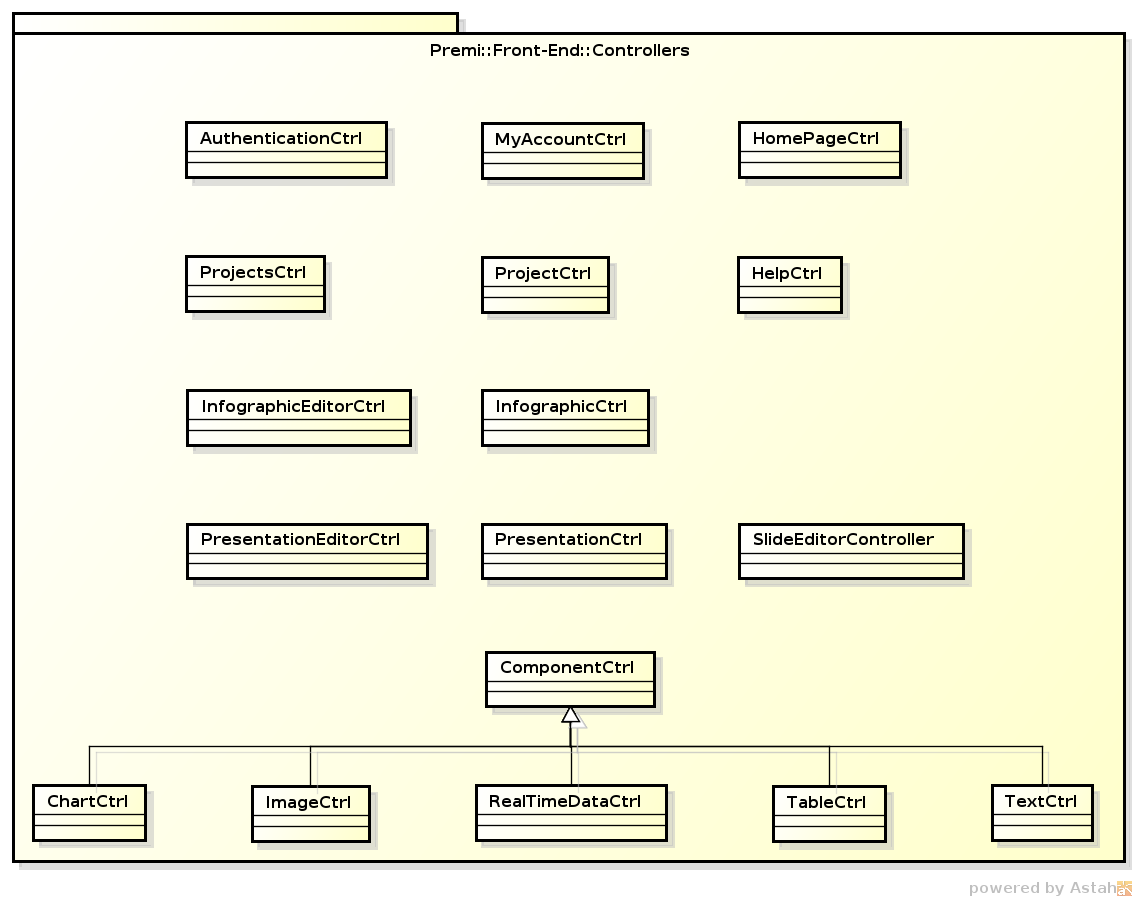
\includegraphics[width=0.7\linewidth]{img/premi_front_end_controllers}
	\caption[Premi::Front-End::Controllers]{Premi::Front-End::Controllers}
\end{figure}
Il package gestisce i controller del front-end dell'applicazione. Comunica con il model, le view e i service della struttura per gestire tutte le operazioni tra di essi. Fa comunicare le view con il model per rendere visibili gli aggiornati effettuati con quest'ultimo e viceversa, aggiorna il model con le informazioni provenienti dalla view. Richiama inoltre i service per comunicare con il back-end e caricare o salvare quindi i dati nel database.
\newpage

\subsubsection{ComponentController}

\newpage

\subsection{Premi::Front-End::Model}
\begin{figure}[h]
	\centering
	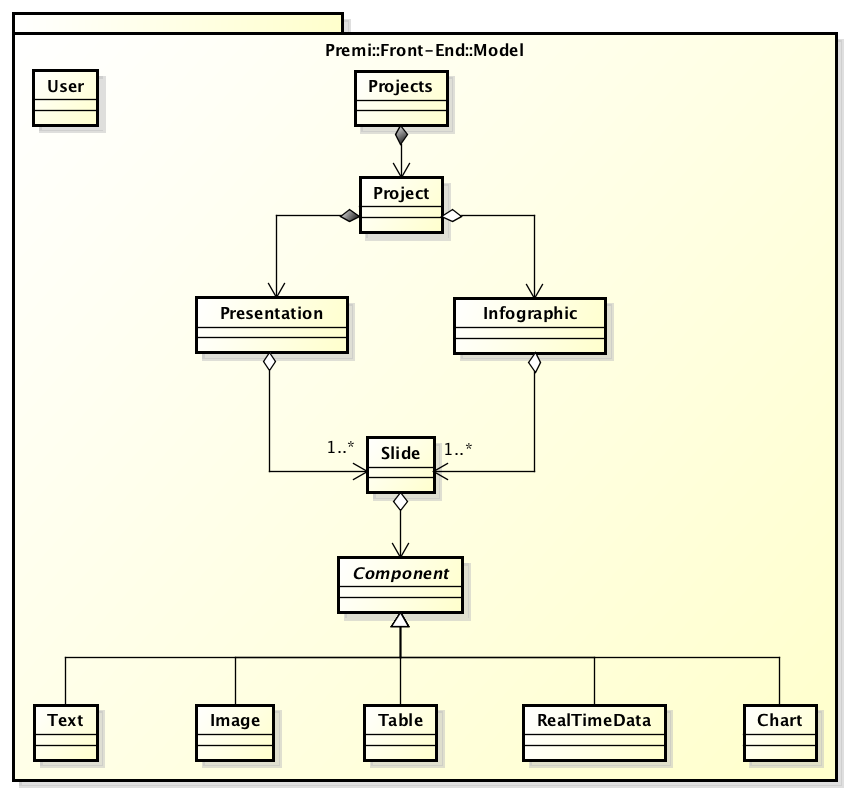
\includegraphics[width=0.7\linewidth]{img/premi_front_end_model}
	\caption[Premi::Front-End::Model]{Premi::Front-End::Model}
\end{figure}
Il package gestisce la memorizzazione delle informazioni dei dati utilizzati nel front-end e la loro logica. Al suo interno è presente una struttura di classi creata per ottimizzare il recupero e il salvataggio di dati anche con il rispettivo model del back-end.
\newpage

\subsection{Premi::Front-End::Directives}
\begin{figure}[h]
	\centering
	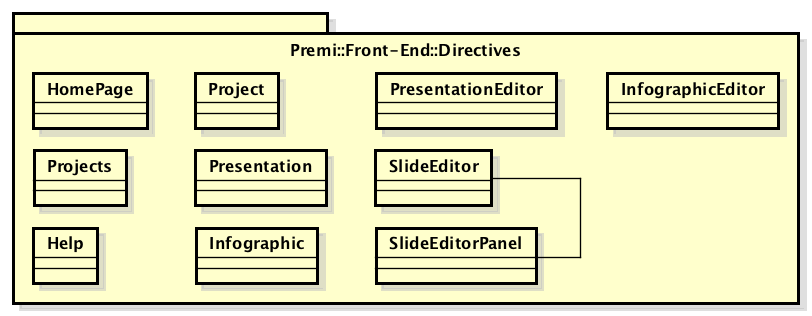
\includegraphics[width=0.7\linewidth]{img/premi_front_end_directives}
	\caption[Premi::Front-End::Directives]{Premi::Front-End::Directives}
\end{figure}
Il package gestisce le direttive del \gls{front-end}. Comunica con le view e con i controller per associarli nel giusto ordine e farli comunicare.
Per brevità nell'identificare una direttiva è stata omessa la dicitura Premi::\gls{Front-End}::Directives lasciando solamente il nome della direttiva stessa. Si assume dunque che la dicitura compatta <nomeDirettiva> rappresenta la forma estesa Premi::\gls{Front-End}::Directives::<nomeDirettiva>.
\newpage


\subsubsection{Help}
	\begin{figure}[h]
		\centering
		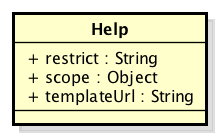
\includegraphics[width=0.4\linewidth]{img/premi_front_end_directives_help}
		\caption[Premi::Front-End::Directives::Help]{Premi::Front-End::Directives::Help}
	\end{figure}
	
	\paragraph{Descrizione}
	Rappresenta il componente grafico che permette di visualizzare gli aiuti agli utenti nelle varie sezioni dell'applicazione.
	
	\paragraph{Utilizzo}
	Viene utilizzata per consentire di far mostrare all'utente i tips nelle sezioni dell'applicazione. Si attiva a seconda dell'opzione selezionata dall'utente, se abilita l'aiuto all'uso dell'applicazione oppure no.
	
	\paragraph{Attributi}
	\begin{itemize}
		\item \textbf{+ controller: String}:\\
			Stringa che specifica il controller da associare alla direttiva. Per questa direttiva è l'\textit{HelpCtrl};
		\item \textbf{+ restrict: String}:\\
			Stringa che specifica la modalità con la quale è possibile inserire la direttiva all'interno della pagina;
		\item \textbf{+ scope: Object}:\\
			Oggetto scope locale della direttiva;
		\item \textbf{+ templateUrl: String}:\\
			Stringa che specifica il percordo dove è situato il file \gls{HTML} che contiene il \gls{template} della direttiva
	\end{itemize}
\newpage


\subsubsection{HomePage}
	\begin{figure}[h]
		\centering
		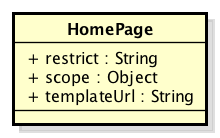
\includegraphics[width=0.4\linewidth]{img/premi_front_end_directives_homepage}
		\caption[Premi::Front-End::Directives::HomePage]{Premi::Front-End::Directives::HomePage}
	\end{figure}
	
	\paragraph{Descrizione}
	Rappresenta il componente grafico che permette all'utente di accedere alle sezioni di login e registrazione e per effettuare la ricerca. Questo componente è visibile all'apertura dell'applicazione.
	
	\paragraph{Utilizzo}
	Viene utilizzata per consentire all'utente di raggiungere le principali sezioni dell'applicazione e per eseguire la ricerca dei progetti. Deve essere inserita nella pagina iniziale del sito e deve essere attivata all'apertura dell'applicazione o nel momento in cui si deve effettuare una ricerca.
		
	\paragraph{Attributi}
	\begin{itemize}
		\item \textbf{+ controller: String}:\\
			Stringa che specifica il controller da associare alla direttiva. Per questa direttiva è l'\textit{HomePageCtrl};
		\item \textbf{+ restrict: String}:\\
			Stringa che specifica la modalità con la quale è possibile inserire la direttiva all'interno della pagina;
		\item \textbf{+ scope: Object}:\\
			Oggetto scope locale della direttiva;
		\item \textbf{+ templateUrl: String}:\\
			Stringa che specifica il percordo dove è situato il file \gls{HTML} che contiene il \gls{template} della direttiva
	\end{itemize}
\newpage
	
	
\subsubsection{InfographicEditor}
	\begin{figure}[h]
		\centering
		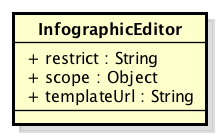
\includegraphics[width=0.4\linewidth]{img/premi_front_end_directives_infographiceditor}
		\caption[Premi::Front-End::Directives::InfographicEditor]{Premi::Front-End::Directives::InfographicEditor}
	\end{figure}
	
	\paragraph{Descrizione}
		Rappresenta il componente grafico che permette all'utente di accedere alla sezione per la gestione delle infografiche di un progetto.
	
	\paragraph{Utilizzo}
	Viene utilizzata per consentire all'utente di gestire le proprie infografiche, visualizzarle, modificarle e crearne di nuove. Deve essere inserita nella pagina relativa ai progetti di un utente e attivata quando è selezionata un'\gls{infografica} dalla pagina stessa.
	
	\paragraph{Attributi}
	\begin{itemize}
		\item \textbf{+ controller: String}:\\
			Stringa che specifica il controller da associare alla direttiva. Per questa classe èl'\textit{InfographicCtrl};
		\item \textbf{+ restrict: String}:\\
			Stringa che specifica la modalità con la quale è possibile inserire la direttiva all'interno della pagina;
		\item \textbf{+ scope: Object}:\\
			Oggetto scope locale della direttiva;
		\item \textbf{+ templateUrl: String}:\\
			Stringa che specifica il percordo dove è situato il file \gls{HTML} che contiene il \gls{template} della direttiva
	\end{itemize}
\newpage	
	

\subsubsection{Presentation}
	\begin{figure}[h]
		\centering
		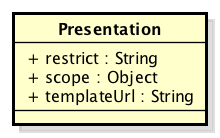
\includegraphics[width=0.4\linewidth]{img/premi_front_end_directives_presentation}
		\caption[Premi::Front-End::Directives::Presentation]{Premi::Front-End::Directives::Presentation}
	\end{figure}
	
	\paragraph{Descrizione}
	Rappresenta il componente grafico che permette all'utente di accedere alla sezione per la visualizzazione di una presentazione.
	
	\paragraph{Utilizzo}
	Viene utilizzata per consentire all'utente di visualizzare una presentazione. Deve essere inserita nella pagina relativa ai progetti di un utente e si deve attivare quando è selezionato il comando show nella pagina dei progetti di un utente oppure dalla pagina dei risultati di ricerca.
	
	\paragraph{Attributi}
	\begin{itemize}
		\item \textbf{+ controller: String}:\\
			Stringa che specifica il controller da associare alla direttiva. Per questa direttiva è il \textit{PresentationCtrl};
		\item \textbf{+ restrict: String}:\\
			Stringa che specifica la modalità con la quale è possibile inserire la direttiva all'interno della pagina;
		\item \textbf{+ scope: Object}:\\
			Oggetto scope locale della direttiva;
		\item \textbf{+ templateUrl: String}:\\
			Stringa che specifica il percordo dove è situato il file \gls{HTML} che contiene il \gls{template} della direttiva
	\end{itemize}
\newpage


\subsubsection{PresentationEditor}
	\begin{figure}[h]
		\centering
		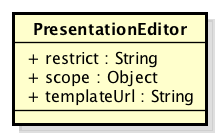
\includegraphics[width=0.4\linewidth]{img/premi_front_end_directives_presentationeditor}
		\caption[Premi::Front-End::Directives::PresentationEditor]{Premi::Front-End::Directives::PresentationEditor}
	\end{figure}
	
	\paragraph{Descrizione}
	Rappresenta il componente grafico che permette all'utente di accedere alla sezione per la modifica di una presentazione.
	
	\paragraph{Utilizzo}
	Viene utilizzata per consentire all'utente di modificare una presentazione. Si attiva quando è selezionato il comando edit nella pagina dei progetti di un utente, deve essere quindi inserita in questa pagina.
	
	\paragraph{Relazione con le altre classi}
	\begin{itemize}
		\item OUT: \textbf{SlideEditor}:\\
		Direttiva che gestisce il componente grafico per la modifica di una \gls{slide}.
	\end{itemize}
	
	\paragraph{Attributi}
	\begin{itemize}
		\item \textbf{+ controller: String}:\\
			Stringa che specifica il controller da associare alla direttiva. Per questa classe è il \textit{PresentationEditorCtrl};
		\item \textbf{+ restrict: String}:\\
			Stringa che specifica la modalità con la quale è possibile inserire la direttiva all'interno della pagina;
		\item \textbf{+ scope: Object}:\\
			Oggetto scope locale della direttiva;
		\item \textbf{+ templateUrl: String}:\\
			Stringa che specifica il percordo dove è situato il file \gls{HTML} che contiene il \gls{template} della direttiva
	\end{itemize}
\newpage


\subsubsection{SlideEditor}
	\begin{figure}[h]
		\centering
		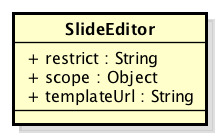
\includegraphics[width=0.4\linewidth]{img/premi_front_end_directives_slideeditor}
		\caption[Premi::Front-End::Directives::SlideEditor]{Premi::Front-End::Directives::SlideEditor}
	\end{figure}
	
	\paragraph{Descrizione}
	Rappresenta il componente grafico che permette all'utente di modificare la \gls{slide} di una presentazione.
	
	\paragraph{Utilizzo}
	Viene utilizzata per consentire all'utente di modificare una \gls{slide} specifica di una presentazione. Si attiva quando viene attivata la direttiva per la modifica di una presentazione. La direttiva \textit{SlideEditor} è inclusa nella componente grafica della direttiva \textit{PresentationEditor}
	
	\paragraph{Relazione con le altre classi}
	\begin{itemize}
		\item IN: \textbf{PresentationEditor}:\\
		Direttiva che gestisce il componente grafico per la modifica di una presentazione.
	\end{itemize}
	
	\paragraph{Attributi}
	\begin{itemize}
		\item \textbf{+ controller: String}:\\
			Stringa che specifica il controller da associare alla direttiva. In questo caso è lo \textit{SlideEditorCtrl};
		\item \textbf{+ restrict: String}:\\
			Stringa che specifica la modalità con la quale è possibile inserire la direttiva all'interno della pagina;
		\item \textbf{+ scope: Object}:\\
			Oggetto scope locale della direttiva;
		\item \textbf{+ templateUrl: String}:\\
			Stringa che specifica il percordo dove è situato il file \gls{HTML} che contiene il \gls{template} della direttiva
	\end{itemize}
\newpage


\subsubsection{Projects}
	\begin{figure}[h]
		\centering
		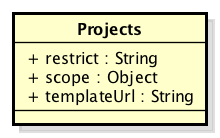
\includegraphics[width=0.4\linewidth]{img/premi_front_end_directives_projects}
		\caption[Premi::Front-End::Directives::Projects]{Premi::Front-End::Directives::Projects}
	\end{figure}
	
	\paragraph{Descrizione}
	Rappresenta il componente grafico che permette all'utente di accedere alla sezione per la visualizzazione dei propri progetti.
	
	\paragraph{Utilizzo}
	Viene utilizzata per consentire all'utente di visualizzare i suoi progetti per poi accedere alle sezioni di presentazione o modifica. Si attiva quando l'utente ha fatto il login e entra nella sua area riservata.
	
	\paragraph{Attributi}
	\begin{itemize}
		\item \textbf{+ controller: String}:\\
			Stringa che specifica il controller da associare alla direttiva. Per questa direttiva è il \textit{ProjectsCtrl};
		\item \textbf{+ restrict: String}:\\
			Stringa che specifica la modalità con la quale è possibile inserire la direttiva all'interno della pagina;
		\item \textbf{+ scope: Object}:\\
			Oggetto scope locale della direttiva;
		\item \textbf{+ templateUrl: String}:\\
			Stringa che specifica il percordo dove è situato il file \gls{HTML} che contiene il \gls{template} della direttiva
	\end{itemize}
\newpage


\subsubsection{User}
	\begin{figure}[h]
		\centering
		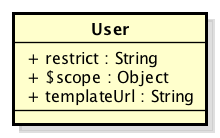
\includegraphics[width=0.4\linewidth]{img/premi_front_end_directives_user}
		\caption[Premi::Front-End::Directives::User]{Premi::Front-End::Directives::User}
	\end{figure}
	
	\paragraph{Descrizione}
	Rappresenta il componente grafico che permette all'utente di accedere alla sezione per la visualizzazione dei propri dati.
	
	\paragraph{Utilizzo}
	Viene utilizzata per consentire all'utente di visualizzare i propri dati. Si attiva nel momento in cui viene eseguito il login al sito.
	
	\paragraph{Attributi}
	\begin{itemize}
		\item \textbf{+ restrict: String}:\\
			Stringa che specifica la modalità con la quale è possibile inserire la direttiva all'interno della pagina;
		\item \textbf{+ scope: Object}:\\
			Oggetto scope locale della direttiva;
		\item \textbf{+ templateUrl: String}:\\
			Stringa che specifica il percordo dove è situato il file \gls{HTML} che contiene il \gls{template} della direttiva
	\end{itemize}
\newpage

\newpage

\subsection{Premi::Front-End::Services}
\begin{figure}[h]
	\centering
	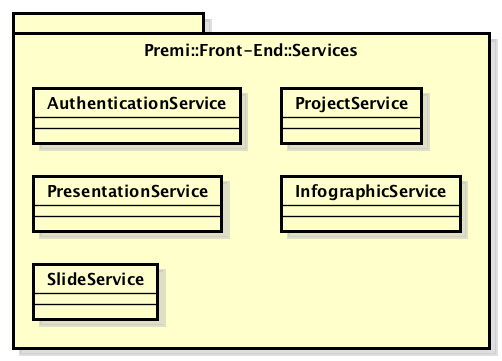
\includegraphics[width=0.7\linewidth]{img/premi_front_end_services}
	\caption[Premi::Front-End::Services]{Premi::Front-End::Services}
\end{figure}
Il package gestisce i services del front-end dell'applicazione. Comunica con i controller e con i servizi REST offerti dal lato back-end, fornendo delle risorse sulle quali creare le funzioni per comunicare tra i due layer. La struttura prevede cinque service principali i quali al loro interno contengono dei metodi specifici che forniscono le risorse per dei servizi più precisi.
Per brevità nell'identificare un service è stata omessa la dicitura Premi::Front-End::Services lasciando solamente il nome del service stesso. Si assume dunque che la dicitura compatta <nomeService> rappresenta la forma estesa Premi::Front-End::Services::<nomeService>.
\newpage


\subsubsection{AuthenticationService}
L'AuthenticationService è una classe che fornisce ulteriori metodi per gestire le funzioni di autenticazione al sito e di gestione degli utenti. Mette a disposizione ulteriori servizi con il compito di creare delle risorse utilizzabili dai metodi creati nei controller per la gestione del login, logout e della registrazione, la gestione dei dati utente e il recupero delle credenziali.

		\subsubsection{AuthenticationService::forgotPasswordService}
		\begin{figure}[h]
			\centering
				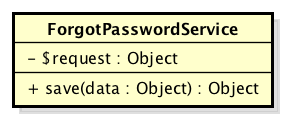
\includegraphics[width=0.4\linewidth]{img/premi_front_end_services_forgotpasswordservice}
			\caption[Premi::Front-End::Services::ForgotPasswordService]{Premi::Front-End::Services::ForgotPasswordService}
		\end{figure}
		
		\paragraph{Descrizione}
		Si occupa di gestire il processo di recupero password per l'autenticazione dell'utente.
		
		\paragraph{Utilizzo}
		Viene utilizzato per creare una risorsa collegata al servizio REST che permette il recupero della password dell'utente.
		
		\paragraph{Relazioni con le altre classi}
		\begin{itemize}
			\item OUT: \textbf{AuthenticationCtrl}:\\
			Classe che gestisce le operazioni per l'autenticazione dell'utente al sistema.
		\end{itemize}
		
		\paragraph{Attributi}
		\begin{itemize}
			\item \textbf{- \$request: Object}:\\
			Campo dati contenente la route per la chiamata al servizio REST specifico del servizio.
		\end{itemize}	
		
		\paragraph{Metodi}
		\begin{itemize}
			\item \textbf{+ save(data: Object)}:\\
			Metodo che richiama la funzione PUT collegata alla risorsa e permette di eseguire la chiamata alla funzione definita nella parte di backend la quale avvia il processo di recupero password, inviando una mail all'indirizzo passato attraverso il parametro della funzione.\\
			\textbf{Parametri:}\\
			\begin{itemize}
				\item \textit{data: Object}: parametro di un oggetto JSON che contiene l'indirizzo email inserito nella view.
			\end{itemize}
		\end{itemize}
\newpage
		
		
		\subsubsection{AuthenticationService::loginService}
		\begin{figure}[h]
			\centering
				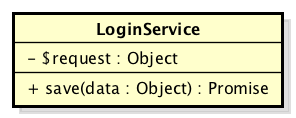
\includegraphics[width=0.4\linewidth]{img/premi_front_end_services_loginservice}
			\caption[Premi::Front-End::Services::LoginService]{Premi::Front-End::Services::LoginService}
		\end{figure}
		
		\paragraph{Descrizione}
		Si occupa di gestire il processo di login dell'utente.
		
		\paragraph{Utilizzo}
		Viene utilizzato per creare una risorsa collegata al servizio REST che permette l'autenticazione dell'utente al sistema.
		
		\paragraph{Relazioni con le altre classi}
		\begin{itemize}
			\item OUT: \textbf{AuthenticationCtrl}:\\
			Classe che gestisce le operazioni per l'autenticazione dell'utente al sistema.
		\end{itemize}
		
		\paragraph{Attributi}
		\begin{itemize}
			\item \textbf{- \$request: Object}:\\
			Campo dati contenente la route per la chiamata al servizio REST specifico del servizio.
		\end{itemize}	
		
		\paragraph{Metodi}
		\begin{itemize}
			\item \textbf{+ save(data: Object): Promise}:\\
			Metodo che richiama la funzione PUT collegata alla risorsa e permette di eseguire il login dell'utente al sistema. Il metodo ritorna una promessa la quale, se ha esito positivo, verrà analizzata per ottenere lo username dell'utente o il messaggio di errore. \\
			\textbf{Parametri:}\\
			\begin{itemize}
				\item \textit{data: Object}: parametro di un oggetto JSON che contiene il nome utente e la password inseriti nella view e necessari per l'autenticazione al sistema.
			\end{itemize}
		\end{itemize}
\newpage
		
		
		\subsubsection{AuthenticationService::logoutService}
		\begin{figure}[h]
			\centering
				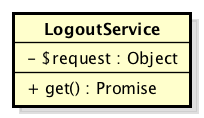
\includegraphics[width=0.4\linewidth]{img/premi_front_end_services_logoutservice}
			\caption[Premi::Front-End::Services::LogoutService]{Premi::Front-End::Services::LogoutService}
		\end{figure}
		
		\paragraph{Descrizione}
		Si occupa di gestire il processo di logout dell'utente.
		
		\paragraph{Utilizzo}
		Viene utilizzato per creare una risorsa collegata al servizio REST che permette l'autenticazione dell'utente al sistema.
		
		\paragraph{Relazioni con le altre classi}
		\begin{itemize}
			\item OUT: \textbf{AuthenticationCtrl}:\\
			Classe che gestisce le operazioni per l'autenticazione dell'utente al sistema.
		\end{itemize}
		
		\paragraph{Attributi}
		\begin{itemize}
			\item \textbf{- \$request: Object}:\\
			Campo dati contenente la route per la chiamata al servizio REST specifico del servizio.
		\end{itemize}	
		
		\paragraph{Metodi}
		\begin{itemize}
			\item \textbf{+ get(): Promise}:\\
			Metodo che richiama la funzione GET collegata alla risorsa e permette di eseguire il logout dell'utente. Il metodo ritorna una promessa e porta all'aggiornamento della pagina per il reset delle variabili si \$scope.
		\end{itemize}
\newpage
		
		
		\subsubsection{AuthenticationService::signUpService}
		\begin{figure}[h]
			\centering
				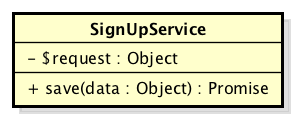
\includegraphics[width=0.4\linewidth]{img/premi_front_end_services_signupservice}
			\caption[Premi::Front-End::Services::SignupService]{Premi::Front-End::Services::SignupService}
		\end{figure}
		
		\paragraph{Descrizione}
		Si occupa di gestire il processo di registrazione dell'utente.
		
		\paragraph{Utilizzo}
		Viene utilizzato per creare una risorsa collegata al servizio REST che permette l'autenticazione dell'utente al sistema.
		
		\paragraph{Relazioni con le altre classi}
		\begin{itemize}
			\item OUT: \textbf{AuthenticationCtrl}:\\
			Classe che gestisce le operazioni per l'autenticazione dell'utente al sistema.
		\end{itemize}
		
		\paragraph{Attributi}
		\begin{itemize}
			\item \textbf{- \$request: Object}:\\
			Campo dati contenente la route per la chiamata al servizio REST specifico del servizio.
		\end{itemize}	
		
		\paragraph{Metodi}
		\begin{itemize}
			\item \textbf{+ save(data: Object): Promise}:\\
			Metodo che richiama la funzione PUT collegata alla risorsa e permette di eseguire la registrazione dell'utente al sistema. Il metodo ritorna una promessa la quale, se la chiamata ha esito positivo, verrà analizzata per ottenere la conferma di avvenuta registrazione o altrimenti, l'array contenenti gli errori commessi nell'inserimento dei dati.\\
			\textbf{Parametri:}\\
			\begin{itemize}
				\item \textit{data: Object}: parametro di un oggetto JSON che contiene tutte le credenziali necessarie inserite nella view per registrarsi come nuovo utente al sistema.
			\end{itemize}
		\end{itemize}
\newpage
		
		
		\subsubsection{AuthenticationService::userService}
		\begin{figure}[h]
			\centering
				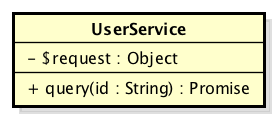
\includegraphics[width=0.4\linewidth]{img/premi_front_end_services_userservice}
			\caption[Premi::Front-End::Services::UserService]{Premi::Front-End::Services::UserService}
		\end{figure}
		
		\paragraph{Descrizione}
		Si occupa di gestire le operazioni riguardanti un utente.
		
		\paragraph{Utilizzo}
		Viene utilizzato per creare una risorsa collegata al servizio REST che permette di gestire le operazioni riguardanti un utente, quali il recupero dei suoi dati.
		
		\paragraph{Relazioni con le altre classi}
		\begin{itemize}
			\item OUT: \textbf{MyAccountCtrl}:\\
			Classe che gestisce la rappresentazione dei dati di un utente.
		\end{itemize}
		
		\paragraph{Attributi}
		\begin{itemize}
			\item \textbf{- \$request: Object}:\\
			Campo dati contenente la route per la chiamata al servizio REST specifico del servizio.
		\end{itemize}	
		
		\paragraph{Metodi}
		\begin{itemize}
			\item \textbf{+ query(id:String): Promise}:\\
			Metodo che richiama la funzione GET collegata alla risorsa e permette di ottenere i dati relativi all'utente con id passato come parametro. Il metodo ritorna una promessa contenete tutti i dati dell'utente
			\textbf{Parametri:}\\
			\begin{itemize}
				\item \textit{id: String}: parametro di una stringa contenente l'id dell'utente.
			\end{itemize}
		\end{itemize}
\newpage


\subsubsection{InfographicService}
L'InfographicService è una classe che mette a disposizione dei metodi per la gestione delle infografiche di un progetto. Con questi metodi è possibile creare delle risorse con le quali si possono creare, modificare o eliminare delle infografiche.

		
		\subsubsection{InfographicService::infographicEditorService}
		\begin{figure}[h]
			\centering
				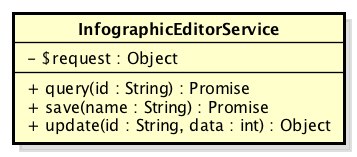
\includegraphics[width=0.4\linewidth]{img/premi_front_end_services_infographiceditorservice}
			\caption[Premi::Front-End::Services::InfographicEditorService]{Premi::Front-End::Services::infographicEditorService}
		\end{figure}
		
		\paragraph{Descrizione}
		Si occupa di gestire le operazioni riguardanti le infografiche del progetto.
		
		\paragraph{Utilizzo}
		Viene utilizzato per creare una risorsa collegata al servizio REST che permette di gestire le operazioni sulle infografiche, quali la crezione, la modifica, il salvataggio e l'eliminazione.
		
		\paragraph{Relazioni con le altre classi}
		\begin{itemize}
			\item OUT: \textbf{InfographicEditorCtrl}:\\
			Classe che gestisce le operazioni di modifica di una infografica.
		\end{itemize}
		
		\paragraph{Attributi}
		\begin{itemize}
			\item \textbf{- \$request: Object}:\\
			Campo dati contenente la route per la chiamata al servizio REST specifico del servizio.
		\end{itemize}	
		
		\paragraph{Metodi}
		\begin{itemize}
			\item \textbf{+ query(id: String): Promise}:\\
				Metodo che richiama la funzione GET collegata alla risorsa e permette di caricare l'infografica richiesta dal database. Il metodo ritorna una promessa la quale, se la chiamata ha esito positivo, conterrà l'infografica con tutti i propri dati.\\
			\item \textbf{+ save(name: String): Promise}:\\
				Metodo che richiama la funzione POST collegata alla risorsa e permette di creare una nuova infografica e di salvarla nel database. Il metodo ritorna una promessa la quale, se la chiamata ha esito positivo, conterrà il valore \textit{true}.\\
			\item \textbf{+ update(id: String, data:Object): Promise}:\\
				Metodo che richiama la funzione PUT collegata alla risorsa e permette di salvare l'infografica aggiornando i dati passati per parametro. Il metodo ritorna una promessa la quale, se la chiamata ha esito positivo, conterrà il valore \textit{true}.\\
			\textbf{Parametri:}\\
			\begin{itemize}
				\item \textit{id: String}: parametro di una stringa contenente l'id dell'infografica sulla quale eseguire le operazioni;
				\item \textit{name: String}: parametro di una stringa contenente il nome dell'infografica da creare;
				\item \textit{data: Object}: parametro di una oggetto contenente i dati necessari per aggiornare l'infografica.
			\end{itemize}
		\end{itemize}
\newpage


\subsubsection{PresentationService}
Il PresentationService rende disponibili dei servizi che si occupano della gestione di una presentazione. Con le risorse che si possono creare, è possibile visualizzare una presentazione oppure modificarla attraverso le opportune chiamate eseguite nella sezione dell'editor.


		\subsubsection{PresentationService::presentationService}
		\begin{figure}[h]
			\centering
				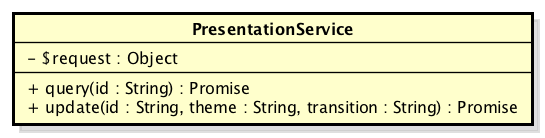
\includegraphics[width=0.5\linewidth]{img/premi_front_end_services_presentationservice}
			\caption[Premi::Front-End::Services::PresentationService]{Premi::Front-End::Services::PresentationService}
		\end{figure}
		
		\paragraph{Descrizione}
		Si occupa di gestire le operazioni riguardanti la presentazione di un progetto.
		
		\paragraph{Utilizzo}
		Viene utilizzato per creare una risorsa collegata al servizio REST che permette di gestire le operazioni sulle presentazioni, cioè di caricarle dal backend oppure di salvarle nel database.
		
		\paragraph{Relazioni con le altre classi}
		\begin{itemize}
			\item OUT: \textbf{PresentationCtrl}:\\
			Classe che gestisce le operazioni di visualizzazione di una presentazione;
			\item OUT: \textbf{PresentationEditorCtrl}:\\
			Classe che gestisce le operazioni modifica di una presentazione.
		\end{itemize}
		
		\paragraph{Attributi}
		\begin{itemize}
			\item \textbf{- \$request: Object}:\\
			Campo dati contenente la route per la chiamata al servizio REST specifico del servizio.
		\end{itemize}	
		
		\paragraph{Metodi}
		\begin{itemize}
			\item \textbf{+ query(id: String): Promise}:\\
			Metodo che richiama la funzione GET collegata alla risorsa e permette di caricare la presentazione dal database. Il metodo ritorna una promessa la quale, se la chiamata ha esito positivo, conterrà la presentazione con tutte le rispettive slide.\\
			\item \textbf{+ update(id: String, theme:String, transition:String): Promise}:\\
			Metodo che richiama la funzione POST collegata alla risorsa e permette di salvare la presentazione aggiornando i dati, anche quelli riguardanti il tema e la transizione tra le slide passati per parametro. Il metodo ritorna una promessa la quale, se la chiamata ha esito positivo, conterrà il valore \textit{true}.\\
			\textbf{Parametri:}\\
			\begin{itemize}
				\item \textit{id: String}: parametro di una stringa contenente l'id della presentazione sulla quale eseguire le operazioni;
				\item \textit{theme: String}: parametro di una stringa contenente il nome del tema da applicare alla presentazione;
				\item \textit{transition: String}: parametro di una stringa contenente il nome della transizione da applicare alla presentazione.
			\end{itemize}
		\end{itemize}
\newpage


\subsubsection{ProjectService}
ProjectService è una classe che mette a disposizione i metodi per l'organizzazione di un progetto. Con le risorse create da questi, è possibile caricare e salvare un progetto già presente nel database, eliminarlo oppure crearne uno di nuovo inserendo i parametri opportuni.

		\subsubsection{ProjectService::projectsService}
		\begin{figure}[h]
			\centering
				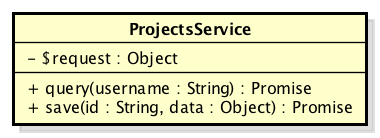
\includegraphics[width=0.4\linewidth]{img/premi_front_end_services_projectsservice}
			\caption[Premi::Front-End::Services::ProjectsService]{Premi::Front-End::Services::ProjectsService}
		\end{figure}
		
		\paragraph{Descrizione}
		Si occupa di gestire le operazioni riguardanti i progetti.
		
		\paragraph{Utilizzo}
		Viene utilizzato per creare una risorsa collegata al servizio REST che permette di gestire le operazioni sui progetti, cioè di caricarli o eliminarli dal database.
		
		\paragraph{Relazioni con le altre classi}
		\begin{itemize}
			\item OUT: \textbf{MyProjectsCtrl}:\\
			Classe che gestisce le operazioni riguardanti i progetti personali di un utente;
			\item OUT: \textbf{ProjectCtrl}:\\
			Classe che gestisce le operazioni riguardanti i progetti;
			\item OUT: \textbf{SearchCtrl}:\\
			Classe che gestisce le operazioni di ricerca. Viene usato per caricare i progetti trovati.
		\end{itemize}
		
		\paragraph{Attributi}
		\begin{itemize}
			\item \textbf{- \$request: Object}:\\
			Campo dati contenente la route per la chiamata al servizio REST specifico del servizio.
		\end{itemize}	
		
		\paragraph{Metodi}
		\begin{itemize}
			\item \textbf{+ query(username: String): Promise}:\\
			Metodo che richiama la funzione GET collegata alla risorsa e permette di caricare i progetti dell'utente con username passato per parametro e i rispettivi contenuti dal database. Il metodo ritorna una promessa la quale, se la chiamata ha esito positivo, conterrà un oggetto avente il progetto e i suoi dati.\\
			\item \textbf{+ save(id: String, data:Object): Promise}:\\
			Metodo che richiama la funzione POST collegata alla risorsa e permette di creare un nuovo progetto con i dati passati per parametro. Il metodo ritorna una promessa la quale, se la chiamata ha esito positivo, conterrà il valore \textit{true}.\\
			\textbf{Parametri:}\\
			\begin{itemize}
				\item \textit{username: String}: parametro di una stringa contenente lo username dell'utente;
				\item \textit{id: String}: parametro di una stringa contenente l'id del progetto sul quale eseguire le operazioni;
				\item \textit{data: Object}: parametro di un oggetto contenente i dati necessari per creare il progetto, quali ad esempio il nome.
			\end{itemize}
		\end{itemize}
\newpage
		
		
		\subsubsection{ProjectService::searchByProjectService}
		\begin{figure}[h]
			\centering
				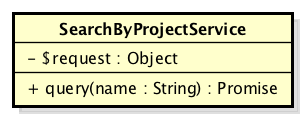
\includegraphics[width=0.4\linewidth]{img/premi_front_end_services_searchbyprojectservice}
			\caption[Premi::Front-End::Services::SearchByProjectService]{Premi::Front-End::Services::SearchByProjectService}
		\end{figure}
		
		\paragraph{Descrizione}
		Si occupa di gestire il processo di ricerca del sistema.
		
		\paragraph{Utilizzo}
		Viene utilizzato per creare una risorsa collegata al servizio REST che permette la ricerca nel sistema attraverso il nome del progetto.
		
		\paragraph{Relazioni con le altre classi}
		\begin{itemize}
			\item OUT: \textbf{HomePageCtrl}:\\
			Classe che gestisce le operazioni di reindirizzamento tra le pagine dall'applicazione e le operazioni di ricerca.
		\end{itemize}
		
		\paragraph{Attributi}
		\begin{itemize}
			\item \textbf{- \$request: Object}:\\
			Campo dati contenente la route per la chiamata al servizio REST specifico del servizio.
		\end{itemize}	
		
		\paragraph{Metodi}
		\begin{itemize}
			\item \textbf{+ query(name: String): Promise}:\\
			Metodo che richiama la funzione GET collegata alla risorsa e permette di eseguire la ricerca nel sistema attraverso il nome di un progetto. Il metodo ritorna una promessa la quale, se la chiamata ha esito positivo, conterrà un array con i dati relativi ai progetti risultato della ricerca.\\
			\textbf{Parametri:}\\
			\begin{itemize}
				\item \textit{name: String}: parametro di una stringa contenente il nome del progetto da cercare inserito nella view.
			\end{itemize}
		\end{itemize}
\newpage
		
		
		\subsubsection{ProjectService::searchByUserService}
		\begin{figure}[h]
			\centering
				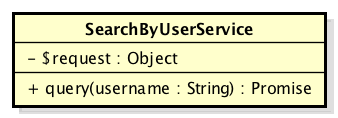
\includegraphics[width=0.4\linewidth]{img/premi_front_end_services_searchbyuserservice}
			\caption[Premi::Front-End::Services::SearchByUserService]{Premi::Front-End::Services::SearchByUserService}
		\end{figure}
		
		\paragraph{Descrizione}
		Si occupa di gestire il processo di ricerca del sistema.
		
		\paragraph{Utilizzo}
		Viene utilizzato per creare una risorsa collegata al servizio REST che permette la ricerca nel sistema attraverso il nome utente.
		
		\paragraph{Relazioni con le altre classi}
		\begin{itemize}
			\item OUT: \textbf{HomePageCtrl}:\\
			Classe che gestisce le operazioni di reindirizzamento tra le pagine dall'applicazione e le operazioni di ricerca.
		\end{itemize}
		
		\paragraph{Attributi}
		\begin{itemize}
			\item \textbf{- \$request: Object}:\\
			Campo dati contenente la route per la chiamata al servizio REST specifico del servizio.
		\end{itemize}	
		
		\paragraph{Metodi}
		\begin{itemize}
			\item \textbf{+ query(username: String): Promise}:\\
			Metodo che richiama la funzione GET collegata alla risorsa e permette di eseguire la ricerca nel sistema attraverso lo username di un utente. Il metodo ritorna una promessa la quale, se la chiamata ha esito positivo, conterrà un array con gli utenti risultato della ricerca, ognuno dei quali avrà le informazioni necessarie per recuperare i rispettivi progetti da analizzare.\\
			\textbf{Parametri:}\\
			\begin{itemize}
				\item \textit{username: String}: parametro di una stringa contenente il nome utente da cercare inserito nella view.
			\end{itemize}
		\end{itemize}
\newpage
		
		
		\subsubsection{ProjectService::projectService}
		\begin{figure}[h]
			\centering
				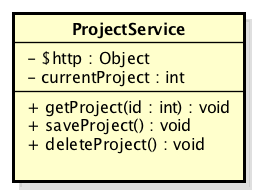
\includegraphics[width=0.4\linewidth]{img/premi_front_end_services_projectservice}
			\caption[Premi::Front-End::Services::ProjectService]{Premi::Front-End::Services::ProjectService}
		\end{figure}
		
		\paragraph{Descrizione}
		Si occupa di gestire le operazioni riguardanti uno specifico progetto di un utente.
		
		\paragraph{Utilizzo}
		Viene utilizzato per creare una risorsa collegata al servizio REST che permette di gestire le operazioni sul progetto, cioè di caricarlo o eliminarli dal database.
		
		\paragraph{Relazioni con le altre classi}
		\begin{itemize}
			\item OUT: \textbf{ProjectCtrl}:\\
			Classe che gestisce le operazioni riguardanti i progetti;
		\end{itemize}
		
		\paragraph{Attributi}
		\begin{itemize}
			\item \textbf{- \$request: Object}:\\
			Campo dati contenente la route per la chiamata al servizio REST specifico del servizio.
		\end{itemize}	
		
		\paragraph{Metodi}
		\begin{itemize}
			\item \textbf{+ delete(id: String): Promise}:\\
			Metodo che richiama la funzione DELETE collegata alla risorsa e permette di rimuovere il progetto e tutto il suo contenuto dal database. Il metodo ritorna una promessa la quale, se la chiamata ha esito positivo, conterrà il valore \textit{true}.\\
			\item \textbf{+ update(id: String, data:Object): Promise}:\\
			Metodo che richiama la funzione PUT collegata alla risorsa e permette di aggiornare i dati del progetto passati per parametro. Il metodo ritorna una promessa la quale, se la chiamata ha esito positivo, conterrà il valore \textit{true}.\\
			\textbf{Parametri:}\\
			\begin{itemize}
				\item \textit{id: String}: parametro di una stringa contenente l'id del progetto sul quale eseguire le operazioni;
				\item \textit{data: Object}: parametro di un oggetto contenente i dati del progetto da aggiornare.
			\end{itemize}
		\end{itemize}
\newpage


\subsubsection{SlideService}
SlideService è l'ultimo dei macro servizi offerti e si occupa della gestione delle slide che compongono una presentazione. Con i metodi che mette a disposizione vengono create delle risorse apposite adatte a gestire tutte le operazioni che è possibile eseguire in una slide.


		\subsubsection{SlideService::indexService}
		\begin{figure}[h]
			\centering
				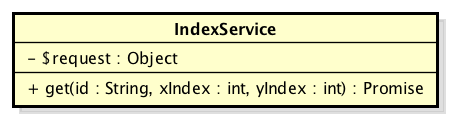
\includegraphics[width=0.4\linewidth]{img/premi_front_end_services_indexservice}
			\caption[Premi::Front-End::Services::IndexService]{Premi::Front-End::Services::IndexService}
		\end{figure}
		
		\paragraph{Descrizione}
		Si occupa di gestire le operazioni riguardanti gli indici delle slide.
		
		\paragraph{Utilizzo}
		Viene utilizzato per creare una risorsa collegata al servizio REST che permette di gestire le operazioni riguardanti gli indici delle slide.
		
		\paragraph{Relazioni con le altre classi}
		\begin{itemize}
			\item OUT: \textbf{SlideServiceCtrl}:\\
			Classe che gestisce le operazioni riguardanti le slide di un progetto.
		\end{itemize}
		
		\paragraph{Attributi}
		\begin{itemize}
			\item \textbf{- \$request: Object}:\\
			Campo dati contenente la route per la chiamata al servizio REST specifico del servizio.
		\end{itemize}	
		
		\paragraph{Metodi}
		\begin{itemize}
			\item \textbf{+ get(id: String, xIndex:int, yIndex:int): Promise}:\\
			Metodo che richiama la funzione GET collegata alla risorsa e permette di ottenere la slide avente x e y corrispondenti ai parametri passati. Il metodo ritorna una promessa la quale, se la chiamata ha esito positivo, conterrà un oggetto avente l'id della slide.\\
			\textbf{Parametri:}\\
			\begin{itemize}
				\item \textit{id: String}: parametro di una stringa contenente l'id del progetto sul quale eseguire la funzione;
				\item \textit{xIndex: int}: parametro di un intero rappresentate la coordinata x della slide richiesta;
				\item \textit{yIndex: int}: parametro di un intero rappresentate la coordinata y della slide richiesta.
			\end{itemize}
		\end{itemize}
\newpage
		
		\subsubsection{SlideService::slideService}
		\begin{figure}[h]
			\centering
				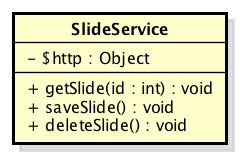
\includegraphics[width=0.5\linewidth]{img/premi_front_end_services_slideservice}
			\caption[Premi::Front-End::Services::SlideService]{Premi::Front-End::Services::SlideService}
		\end{figure}
		
		\paragraph{Descrizione}
		Si occupa di gestire le operazioni di una slide.
		
		\paragraph{Utilizzo}
		Viene utilizzato per creare una risorsa collegata al servizio REST che permette di modificare una slide. Dà la possiblità di creare, caricare, salvare e eliminare una slide dal database.
		
		\paragraph{Relazioni con le altre classi}
		\begin{itemize}
			\item OUT: \textbf{SlideEditorCtrl}:\\
			Classe che gestisce le operazioni di modifica di una slide.
		\end{itemize}
		
		\paragraph{Attributi}
		\begin{itemize}
			\item \textbf{- \$request: Object}:\\
			Campo dati contenente la route per la chiamata al servizio REST specifico del servizio.
		\end{itemize}	
		
		\paragraph{Metodi}
		\begin{itemize}
			\item \textbf{+ get(id:String): Promise}:\\
			Metodo che richiama la funzione GET collegata alla risorsa e permette di ottenere la slide dal backend identificata dall'id passato come parametro. IL metodo ritorna una promessa contenente un oggetto JSON avente tutte le informazioni e i dati riguardanti la slide e i suoi componenti. Questo oggetto è pronto per essere passato all'apposito metodo di caricamento della slide;
			\item \textbf{+ save(xIndex:int, yIndex:int): Promise}:\\
			Metodo che richiama la funzione POST collegata alla risorsa e permette di creare una nuova slide avente le coordinate passate per parametro. Il metodo ritorna una promessa la quale, se la chiamata ha esito positivo, conterrà l'id della nuova slide creata;\\
			\item \textbf{+ update(id:String, xIndex:int, yIndex:int, components:JSON, background:String, slideSVG:SVG):Promise}\\
			Metodo che richiama la funzione PUT collegata alla risorsa e permette di aggiornare una slide già creata (identificata dal parametro id). Con questa chiamata è possibile passare le coordinate aggiornate, i componenti della slide, il colore di sfondo e l'SVG rappresentante la slide stessa. Il metodo ritorna una promessa che conterrà \textit{true} se l'esito del salvataggio è positivo;
			\item \textbf{+ delete(id:String):Promise}\\
			Metodo che richiama la funzione DELETE collegata alla risorsa e permette di eliminare la slide con id passato per parametro. Il metodo ritorna una promessa che conterrà \textit{true} se l'esito del salvataggio è positivo.
			
			\textbf{Parametri:}\\
			\begin{itemize}
				\item \textit{background: String}: parametro di una stringa che contiene il codice del colore di sfondo della slide;
				\item \textit{components: JSON}: parametro di un oggetto JSON contenente tutti i componenti inclusi nella slide;
				\item \textit{id: String}: parametro di una stringa contenente l'id del progetto sul quale eseguire la funzione;
				\item \textit{slideSVG: SVG}: parametro di un oggetto SVG che contiene la rappresentazione della slide in SVG;
				\item \textit{xIndex: int}: parametro di un intero rappresentate la coordinata x della slide richiesta;
				\item \textit{yIndex: int}: parametro di un intero rappresentate la coordinata y della slide richiesta.
			\end{itemize}
		\end{itemize}
\newpage

\subsection{Premi::Front-End::Views}
\begin{figure}[h]
	\centering
	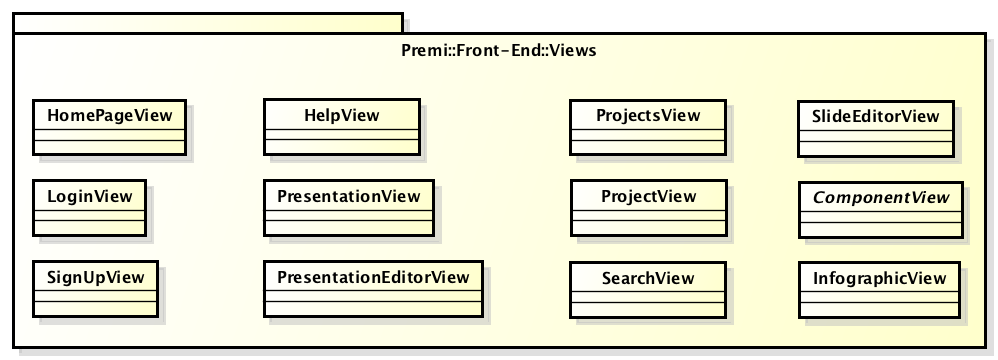
\includegraphics[width=0.7\linewidth]{img/premi_front_end_views}
	\caption[Premi::Front-End::Views]{Premi::Front-End::Views}
\end{figure}
Il package gestisce le view del \gls{front-end} dell'applicazione. Comunica con il model, il controller e le direttive della struttura per acquisire i dati da visualizzare e far ottenere al model i dati modificati dall'utente attraverso il controller. Il package inoltre comunica con i \gls{framework} esterni necessari per la creazione degli oggetti da utilizzare nel programma.

\subsubsection{Component}
	\begin{figure}[h]
		\centering
		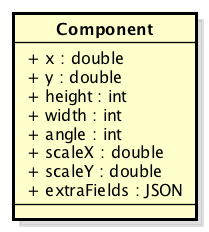
\includegraphics[width=0.3\linewidth]{img/premi_front_end_views_component}
		\caption[Premi::Front-End::Views::Component]{Premi::Front-End::Views::Component}
	\end{figure}
	
	\paragraph{Descrizione}
	Visualizza i componenti che è possibile inserire in una \gls{slide} e le rispettive informazioni.
	
	\paragraph{Utilizzo}
	Viene utilizzata come view per visualizzare e modificare gli attributi di un componente della \gls{slide}. Da essa derivano le view specifiche di ciascun componente.
	
	\paragraph{Relazioni con altre classi}
	\begin{itemize}
		\item \textbf{\textit{IN} ComponentCtrl}:\\
		Classe che gestisce le operazioni generali per la gestione di un componente.
	\end{itemize}
	
	\paragraph{Attributi}
	\begin{itemize}
		\item \textbf{+ x: double}:\\
			Campo dati che contiene la coordinata x di origine del componente;
		\item \textbf{+ y: double}:\\
			Campo dati che contiene la coordinata y di origine del componente;
		\item \textbf{+ height: int}:\\
			Campo dati che contiene la l'altezza del componente;
		\item \textbf{+ width: int}:\\
			Campo dati che contiene la larghezza del componente;
		\item \textbf{+ angle: int}:\\
			Campo dati che contiene l'angolo di rotazione del componente;
		\item \textbf{+ scaleX: duble}:\\
			Campo dati che contiene la scala sull'asse x del componente;
		\item \textbf{+ scaleY: double}:\\
			Campo dati che contiene la scala sull'asse y del componente;
		\item \textbf{+ extraFields: JSON}:\\
			Campo dati che contiene un array \gls{JSON} avente tutti i campi dati secondari di un componente.
	\end{itemize}
\newpage
	

%\subsubsection{Help}
%	\begin{figure}[h]
%		\centering
%		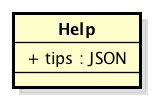
\includegraphics[width=0.3\linewidth]{img/premi_front_end_views_help}
%		\caption[Premi::\gls{Front-End}::Views::Help]{Premi::\gls{Front-End}::Views::Help}
%	\end{figure}
%	
%	\paragraph{Descrizione}
%	View che contiene il tool di aiuto all'utente.
%	
%	\paragraph{Utilizzo}
%	Viene utilizzata come view per visualizzare l'help per l'utente.
%	
%	\paragraph{Relazioni con le altre classi}
%	\begin{itemize}
%		\item \textbf{\textit{IN} HelpCtrl}:\\
%		Classe che gestisce la visualizzazione dell'aiuto all'utente.
%	\end{itemize}
%	
%	\paragraph{Attributi}
%	\begin{itemize}
%		\item \textbf{+ tips:\gls{JSON}}: \\
%		Campo dati che contiene un array \gls{JSON} con tutti gli aiuti da fornire all'utente.
%	\end{itemize}
%\newpage
	
	
\subsubsection{HomePage}
	\begin{figure}[h]
		\centering
		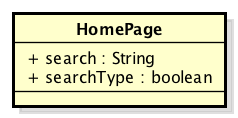
\includegraphics[width=0.3\linewidth]{img/premi_front_end_views_homepage}
		\caption[Premi::Front-End::Views::HomePage]{Premi::Front-End::Views::HomePage}
	\end{figure}
	
	\paragraph{Descrizione}
	Visualizza la pagina principale dell'applicazione.
	
	\paragraph{Utilizzo}
	Viene utilizzata come view per accedere all'area riservata all'utente, alle pagine per il login e la registrazione ed è utilizzata per cercare un utente o un progetto nel sistema attraverso l'apposito form.
	
	\paragraph{Relazioni con le altre classi}
	\begin{itemize}
		\item \textbf{\textit{IN} HomePageCtrl}:\\
			Classe che gestisce la home page e gli accessi alle altre pagine dell'applicazione;
		\item \textbf{\textit{IN} SearchCtrl}:\\
			Classe che gestisce le operazioni di ricerca;
		\item \textbf{\textit{IN} HelpCtrl}:\\
			Classe che gestisce le operazioni per l'aiuto all'utente;
		\item \textbf{\textit{IN} AuthenticationCtrl}:\\
			Classe che gestisce le operazioni per l'autenticazione dell'utente.
	\end{itemize}
	
	\paragraph{Attributi}
	\begin{itemize}
		\item \textbf{+ search: String}:\\
			Campo dati per il contenuto della ricerca da effettuare;
		\item \textbf{+ searchType: boolean}:\\
			Campo dati la scelta del tipo di ricerca da effettuare (per nome utente o per nome del progetto).
	\end{itemize}
\newpage
	
	
\subsubsection{InfographicEditor}
	\begin{figure}[h]
		\centering
		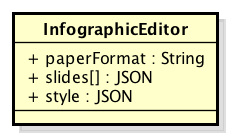
\includegraphics[width=0.3\linewidth]{img/premi_front_end_views_infographiceditor}
		\caption[Premi::Front-End::Views::InfographicEditor]{Premi::Front-End::Views::InfographicEditor}
	\end{figure}
	
	\paragraph{Descrizione}
	Visualizza la pagina per la gestione di un'\gls{infografica}.
	
	\paragraph{Utilizzo}
	Viene utilizzata come view per visualizzare un'\gls{infografica}, modificarla e salvarla.
	
	\paragraph{Relazioni con le altre classi}
	\begin{itemize}
		\item \textbf{\textit{IN} InfographicEditorCtrl}:\\
			Classe che gestisce le operazioni per le infografiche (creazione, modifica, salvataggio);
		\item \textbf{\textit{IN} HelpCtrl}:\\
			Classe che gestisce le operazioni per l'aiuto all'utente.
	\end{itemize}
	
	\paragraph{Attributi}
	\begin{itemize}
		\item \textbf{+ paperFormat: String}:\\
			Campo dati per il formato adottato dall'\gls{infografica};
		\item \textbf{+ slides[]: \gls{JSON}}:\\
			Campo dati contenente l'array di \gls{slide} che compongono l'\gls{infografica};
		\item \textbf{+ style: \gls{JSON}}:\\
		Campo dati per le informazioni dello stile da utilizzare per l'\gls{infografica}.
	\end{itemize}
\newpage
	
	
\subsubsection{Login}
	\begin{figure}[h]
		\centering
		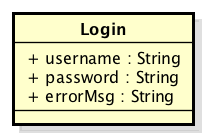
\includegraphics[width=0.3\linewidth]{img/premi_front_end_views_login}
		\caption[Premi::Front-End::Views::Login]{Premi::Front-End::Views::Login}
	\end{figure}
	
	\paragraph{Descrizione}
	View che visualizza il form per inserire i dati necessari al login. Fornisce inoltre un link per il reset della password.
	
	\paragraph{Utilizzo}
	Viene visualizzata dopo aver premuto il rispettivo bottone per permettere l'autenticazione all'utente.
	
	\paragraph{Relazioni con le altre classi}
	\begin{itemize}
		\item \textbf{\textit{IN} LoginCtrl}:\\
		Classe che gestisce le operazioni per l'autenticazione al sito;
		\item \textbf{\textit{IN} AuthenticationCtrl}:\\
		Classe che gestisce le operazioni per l'autenticazione dell'utente.
	\end{itemize}
	
	\paragraph{Attributi}
	\begin{itemize}
		\item \textbf{+ username: String}:\\
		Campo dati contenente lo username dell'utente;
		\item \textbf{+ password: String}:\\
		Campo dati per la password dell'utente;
		\item \textbf{+ errorMsg: String}:\\
		Campo dati contenente l'eventuale messaggio di errore da fornire all'utente.
	\end{itemize}
\newpage


\subsubsection{MyAccount}
	\begin{figure}[h]
		\centering
		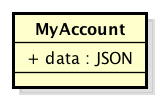
\includegraphics[width=0.3\linewidth]{img/premi_front_end_views_myaccount}
		\caption[Premi::Front-End::Views::MyAccount]{Premi::Front-End::Views::MyAccount}
	\end{figure}
	
	\paragraph{Descrizione}
	View che visualizza le informazioni personali dell'utente.
	
	\paragraph{Utilizzo}
	Viene visualizzata dopo aver eseguito il login per mostrare le informazioni personali dell'utente.
	
	\paragraph{Relazioni con le altre classi}
	\begin{itemize}
		\item \textbf{\textit{IN} MyAccountCtrl}:\\
		Classe che gestisce le operazioni per il recupero dei dati dell'utente.
	\end{itemize}
	
	\paragraph{Attributi}
	\begin{itemize}
		\item \textbf{+ data: JSON}:\\
		Campo dati contenente i dati dell'utente.
	\end{itemize}
\newpage
	
	
\subsubsection{PresentationEditor}
	\begin{figure}[h]
		\centering
		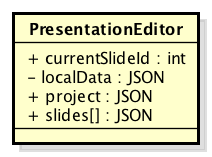
\includegraphics[width=0.3\linewidth]{img/premi_front_end_views_presentationeditor}
		\caption[Premi::Front-End::Views::PresentationEditor]{Premi::Front-End::Views::PresentationEditor}
	\end{figure}
	
	\paragraph{Descrizione}
	Visualizza l'editor di una presentazione.
	
	\paragraph{Utilizzo}
	Viene utilizzata come view per modificare una presentazione e le impostazioni globali di essa. Permette di aggiungere o rimuovere \gls{slide} e di spostarsi tra di esse. Dà la possibilità, inoltre, di accedere alla sezione di modifica di ogni singola \gls{slide}.
	
	\paragraph{Relazioni con le altre classi}
	\begin{itemize}
		\item \textbf{\textit{IN} PresentationEditorCtrl}:\\
		Classe che gestisce le operazioni di modifica delle impostazioni generali della presentazione e le operazioni di spostamento, aggiunta e rimozione di una \gls{slide};
		\item \textbf{\textit{IN} AuthenticationCtrl}:\\
		Classe che gestisce le operazioni per l'autenticazione dell'utente.
	\end{itemize}
	
	\paragraph{Attributi}
	\begin{itemize}
		\item \textbf{+ project: \gls{JSON}}:\\
		Campo dati che contiene le informazioni del progetto corrente;
		\item \textbf{+ slides[]: \gls{JSON}}:\\
		Campo dati che contiene un array \gls{JSON} avente le principali informazioni delle \gls{slide} della presentazione;
		\item \textbf{+ currentSlideId: int}:\\
		Campo dati che contiene l'id della \gls{slide} corrente;
		\item \textbf{- localData: \gls{JSON}}:\\
		Campo dati che contiene le informazioni relative agli indici della \gls{slide} corrente e agli indici massimi della presentazione.
	\end{itemize}
\newpage
	
	
\subsubsection{Presentation}
	\begin{figure}[h]
		\centering
		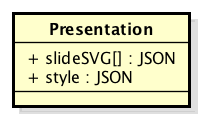
\includegraphics[width=0.3\linewidth]{img/premi_front_end_views_presentation}
		\caption[Premi::Front-End::Views::Presentation]{Premi::Front-End::Views::Presentation}
	\end{figure}
	
	\paragraph{Descrizione}
	Visualizza la pagina di visualizzazione di una presentazione.
	
	\paragraph{Utilizzo}
	Viene utilizzata come view per visualizzare e riprodurre la presentazione, sia come ascoltatore che come presentatore.
	
	\paragraph{Relazioni con le altre classi}
	\begin{itemize}
		\item \textbf{\textit{IN} PresentationCtrl}:\\
			Classe che gestisce le operazioni di recupero dei dati e della visualizzazione della presentazione.
	\end{itemize}
	
	\paragraph{Attributi}
	\begin{itemize}
		\item \textbf{+ slideSVG[]: String}:\\
		Campo dati che contiene un array di stringhe di oggetti SVG rappresentanti le \gls{slide} della presentazione;
		\item \textbf{+ style: JSON}: \\
		Campo dati che contiene un oggetto \gls{JSON} con i dati dello stile della presentazione (tema e effetto di transizione).
	\end{itemize}
\newpage
	
	
\subsubsection{Projects}
	\begin{figure}[h]
		\centering
		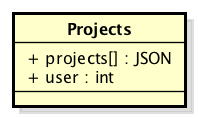
\includegraphics[width=0.3\linewidth]{img/premi_front_end_views_projects}
		\caption[Premi::Front-End::Views::Projects]{Premi::Front-End::Views::Projects}
	\end{figure}
	
	\paragraph{Descrizione}
	Visualizza la pagina con la lista dei progetti di un utente.
	
	\paragraph{Utilizzo}
	Viene utilizzata come view per selezionare i progetti di utente da aprire e per accedere alla funzione di crearne uno nuovo.
	
	\paragraph{Relazioni con le altre classi}
	\begin{itemize}
		\item \textbf{\textit{IN} NewProject}:\\
			Classe che gestisce la creazione di un nuovo progetto;
		\item \textbf{\textit{IN} ProjectsCtrl}:\\
			Classe che gestisce il caricamento dei progetti di un utente e le operazioni che è possibile effettuare su di essi;
		\item \textbf{\textit{IN} HelpCtrl}:\\
		Classe che gestisce le operazioni per l'aiuto all'utente.
	\end{itemize}
	
	\paragraph{Attributi}
	\begin{itemize}
		\item \textbf{+ projects[]: JSON}:\\
			Campo dati che contiene l'array dei progetti dell'utente;
		\item \textbf{+ user: int}:\\
			Campo dati che contiene l'id dell'utente.
	\end{itemize}
\newpage
	
	
\subsubsection{Project}
	\begin{figure}[h]
		\centering
		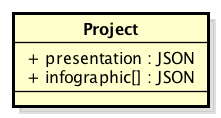
\includegraphics[width=0.3\linewidth]{img/premi_front_end_views_project}
		\caption[Premi::Front-End::Views::Project]{Premi::Front-End::Views::Project}
	\end{figure}
	
	\paragraph{Descrizione}
	Visualizza l'anteprima del progetto selezionato.
	
	\paragraph{Utilizzo}
	Viene utilizzata come view per visualizzare l'anteprima della presentazione e le infografiche di un progetto e per selezionare le operazioni da eseguire su di essi.
	
	\paragraph{Relazioni con le altre classi}
	\begin{itemize}
		\item \textbf{\textit{IN} ProjectsCtrl}:\\
			Classe che gestisce i progetti di un utente;
		\item \textbf{\textit{OUT} PresentationCtrl}:\\
			Classe che gestisce la visualizzazione di una presentazione;
		\item \textbf{\textit{OUT} presentationEditorCtrl}:\\
			Classe che gestisce la modifica di una presentazione;
		\item \textbf{\textit{OUT} infographicEditorCtrl}:\\
			Classe che gestisce le infografiche e la loro modifica;
		\item \textbf{\textit{IN} AuthenticationCtrl}:\\
			Classe che gestisce le operazioni per l'autenticazione dell'utente.
	\end{itemize}
	
	\paragraph{Attributi}
	\begin{itemize}
		\item \textbf{+ presentation: JSON}:\\
			Campo dati che contiene un oggetto \gls{JSON} avente l'id e i dati relativi all'anteprima del progetto;
		\item \textbf{+ infographic[]: JSON}:\\
			Campo dati che contiene un array di oggetti \gls{JSON} aventi gli id e i dati relativi alle infografiche del progetto.
	\end{itemize}
\newpage
	
	
\subsubsection{ResetPassword}
	\begin{figure}[h]
		\centering
		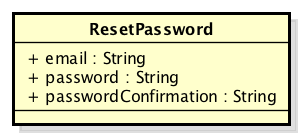
\includegraphics[width=0.3\linewidth]{img/premi_front_end_views_resetpassword}
		\caption[Premi::Front-End::Views::ResetPassword]{Premi::Front-End::Views::ResetPassword}
	\end{figure}
	
	\paragraph{Descrizione}
	View che contiene il form per procedere con il reset della password.
	
	\paragraph{Utilizzo}
	Viene utilizzata come view per resettare la password dopo aver avviato l'apposita procedura di reset.
	
	\paragraph{Relazioni con le altre classi}
	\begin{itemize}
		\item \textbf{\textit{IN} ResetPasswordCtrl}:\\
		Classe che gestisce il reset della password di un utente.
	\end{itemize}
	
	\paragraph{Attributi}
	\begin{itemize}
		\item \textbf{+ email:String}: \\
		Campo dati che contiene l'email dell'utente che deve resettare la password;
		\item \textbf{+ password:String}: \\
		Campo dati che contiene la nuova password per l'utente;
		\item \textbf{+ passwordConfirmation:String}: \\
		Campo dati che contiene la conferma della nuova password per l'utente.
	\end{itemize}
\newpage
	

\subsubsection{Search}
	\begin{figure}[h]
		\centering
		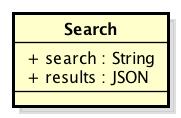
\includegraphics[width=0.3\linewidth]{img/premi_front_end_views_search}
		\caption[Premi::Front-End::Views::Search]{Premi::Front-End::Views::Search}
	\end{figure}
	
	\paragraph{Descrizione}
	View che visualizza i risultati di una ricerca eseguita da un utente, lanciata dalla schermata di home page.
	
	\paragraph{Utilizzo}
	Viene utilizzata come view per visualizzare i risultati di una ricerca.
	
	\paragraph{Relazioni con le altre classi}
	\begin{itemize}
		\item \textbf{\textit{IN} SearchCtrl}:\\
		Classe che gestisce la ricerca per nome utente o per nome del progetto.
	\end{itemize}
	
	\paragraph{Attributi}
	\begin{itemize}
		\item \textbf{+ search: String}:\\
		Campo dati per identificare il nome utente o il nome del progetto da cercare;
		\item \textbf{+ results: JSON}:\\
		Campo dati che contiene un array \gls{JSON} con i risultati della ricerca;
	\end{itemize}
\newpage
	
	
\subsubsection{SignUp}
	\begin{figure}[h]
		\centering
		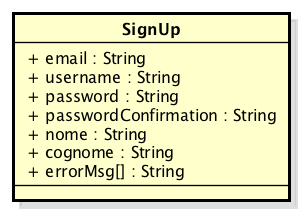
\includegraphics[width=0.3\linewidth]{img/premi_front_end_views_signup}
		\caption[Premi::Front-End::Views::SignUp]{Premi::Front-End::Views::SignUp}
	\end{figure}
	
	\paragraph{Descrizione}
	View che visualizza il form per permettere la registrazione dell'utente al sito.
	
	\paragraph{Utilizzo}
	Viene utilizzata come view per inserire i dati necessari a registrarsi nel sistema.
	
	\paragraph{Relazioni con le altre classi}
	\begin{itemize}
		\item \textbf{\textit{IN} SignUpCtrl}:\\
		Classe che gestisce le operazioni di registrazione al sito;
		\item \textbf{\textit{IN} AuthenticationCtrl}:\\
		Classe che gestisce le operazioni per l'autenticazione dell'utente.
	\end{itemize}
	
	\paragraph{Attributi}
	\begin{itemize}
		\item \textbf{+ email: String}:\\
			Campo dati per l'email dell'utente;
		\item \textbf{+ username: String}:\\
			Campo dati per il nome utente;
		\item \textbf{+ password: String}:\\
			Campo dati per la password dell'utente;
		\item \textbf{+ passwordConfirmation: String}:\\
			Campo dati per la ripetizione della password dell'utente;
		\item \textbf{+ Nome: String}:\\
			Campo dati per il nome dell'utente;
		\item \textbf{+ Cognome: String}:\\
			Campo dati per il cognome dell'utente;		
		\item \textbf{+ errorMsg[]: String}:\\
			Array contenente gli eventuali messaggi di errore da fornire all'utente se i dati non sono inseriti correttamente.
	\end{itemize}
\newpage
	
	
\subsubsection{SlideEditor}
	\begin{figure}[h]
		\centering
		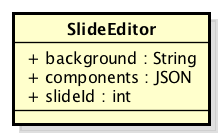
\includegraphics[width=0.3\linewidth]{img/premi_front_end_views_slideeditor}
		\caption[Premi::Front-End::Views::SlideEditor]{Premi::Front-End::Views::SlideEditor}
	\end{figure}
	
	\paragraph{Descrizione}
	Visualizza la sezione dedicata alla modifica di una \gls{slide} della presentazione.
	
	\paragraph{Utilizzo}
	Viene utilizzata come view per modificare una \gls{slide}, permette di inserire i componenti, modificarli secondo i rispettivi parametri e rimuoverli. Permette inoltre di salvare le modifiche effettuate.
	
	\paragraph{Relazioni con le altre classi}
	\begin{itemize}
		\item \textbf{\textit{IN} HelpCtrl}:\\
			Classe che gestisce le operazioni per l'aiuto all'utente;
		\item \textbf{\textit{IN} SlideEditorCtrl}:\\
			Classe che gestisce le operazioni di modifica di una \gls{slide}, la gestione dei suoi componenti e il suo salvataggio;
		\item \textbf{\textit{IN} PresentationEditorCtrl}:\\
			Classe che gestisce le operazioni di modifica delle impostazioni generali della presentazione e le operazioni di spostamento, aggiunta e rimozione di una \gls{slide}.
	\end{itemize}
	
	\paragraph{Attributi}
	\begin{itemize}
		\item \textbf{+ background: String}:\\
			Campo dati per il background della \gls{slide};
		\item \textbf{+ components[]: JSON}:\\
			Campo dati contenente un array con tutti gli elementi presenti nella \gls{slide};
		\item \textbf{+ slideId: int}:\\
			Campo dati per l'id della \gls{slide} corrente.
	\end{itemize}

\newpage

\newpage

\section{Specifica Back-end}
\subsection{Premi::Model}
	\begin{figure}[h]
		\centering
		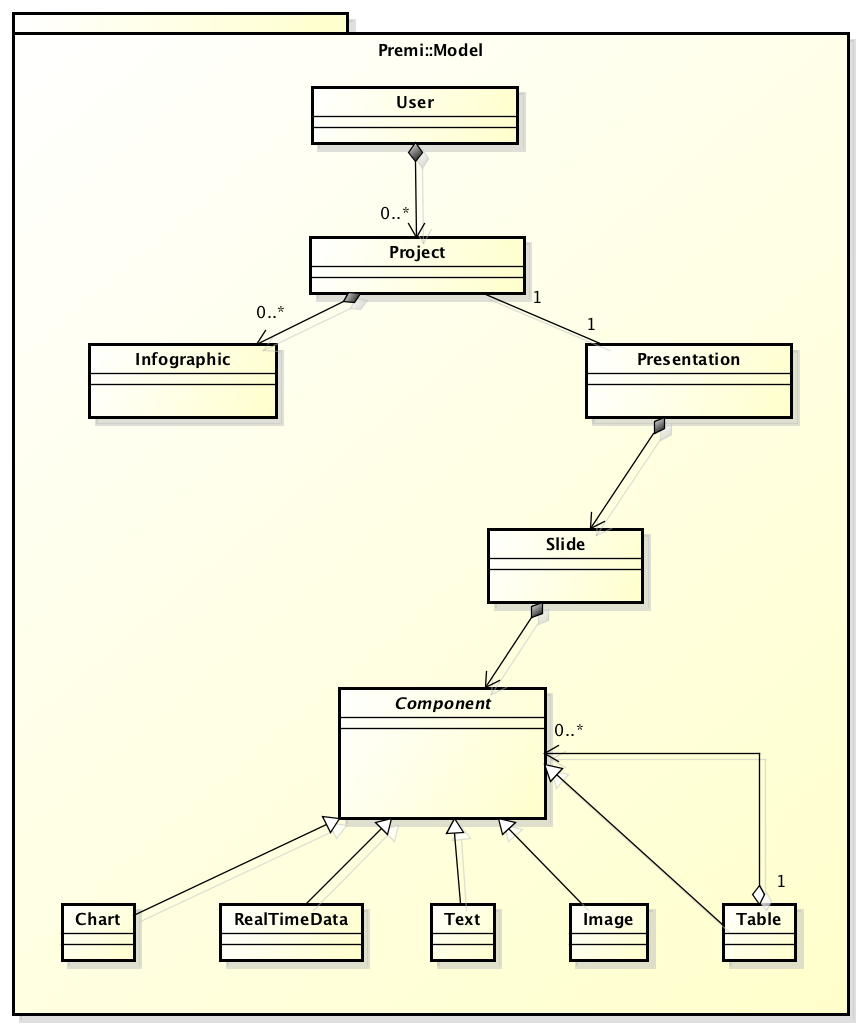
\includegraphics[width=0.7\linewidth]{img/premi_model}
		\caption[Premi::Model]{Premi::Model}
		\label{fig:premi_model}
	\end{figure}
	
Il package gestisce lo scambio di informazioni tra una sorgente dati e l'interfaccia utente, attraverso i controller. Per ottenere informazioni si comunica con il model. Tutti i model comunicano tra di loro andando a costruire una serie di relazioni che rendono più semplice e veloce il recupero dei dati da parte del controller. Laravel utilizza un proprio ORM(Object Relational Mapping) chiamato Eloquent. Tutti i model estendono Eloquent che permette l'integrazione del database con il tipo di programmazione utilizzata.

	\newpage
\subsubsection{User}

	\begin{figure}[h]
		\centering
		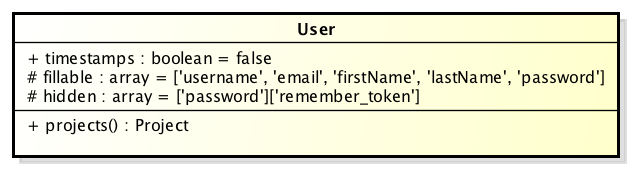
\includegraphics[width=0.7\linewidth]{img/User}
		\caption[Diagramma della classe User]{Diagramma della classe User}
		\label{fig:User}
	\end{figure}

	\subsubsection*{Descrizione}
	Il model User permette di gestire la collection users del database. Eloquent presume che il nome della classe sia il singolare del nome della collection nel database, quindi collega USer alla collection users.
	\subsubsection*{Utilizzo}
	Il model gestisce la collection users del database.
	\subsubsection*{Attributi}
	\begin{itemize}
		\item \textbf{+ timestamps : boolean = false :}\\
		Di default Eloquent automatizza l'inserimento del timestamp relativo all'inserimento e aggiornamento di un campo. Se alla variabile viene assegnato il valore le informazioni dell'inserimento e del aggiornamento non verranno aggiunto alla collection.
		\item \textbf{\# fillable : array = ['username', 'email', 'firstName', 'lastName', 'password']:}\\
		Quando si crea un model, si deve passare una serie di attributi al costruttore del model stesso. Questi attributi vengono assegnati al model tramite \textbf{mass assignment}. La propietà \textit{fillable} serve a specificare quali attributi devono essere assegnabili tramite il mass-assignment.
		\item \textbf{\# hidden : array = ['password', 'remember\_token''] : }\\
		La proprietà hidden si aggiunge quando si vuole limitare gli attributi che sono inclusi nel JSON.
	\end{itemize}
	\subsubsection*{Metodi}
	\begin{itemize}
		\item \textbf{+ projects() : Project}\\
		Abbiamo utilizzato la relazione embedsMany per riuscire ad incorporare il model projects all'interno dell'oggetto principale User. Il metodo ritorna Project su cui verrà chiamato il metodo save() nel caso in cui si voglia aggiornare il modello.
	\end{itemize}
	
\newpage
\subsubsection{Project}

%figura

	\subsubsection*{Descrizione}
	Il model Project rappresenta un progetto creato da un utente. Contiene la presentazio e una o
più infografiche create da esso o nessuna.

	\subsubsection*{Utilizzo}
	Viene utilizzato alla creazione o caricamento di un progetto.
	
	\subsubsection*{Attributi}
	\begin{itemize}
		\item \textbf{+ timestamps : boolean = false :}\\
		Di default Eloquent automatizza l'inserimento del timestamp relativo all'inserimento e aggiornamento di un campo. Se alla variabile viene assegnato il valore le informazioni dell'inserimento e del aggiornamento non verranno aggiunto alla collection.
		\item \textbf{\# fillable : array = [’name’]:}\\
		Quando si crea un model, si deve passare una serie di attributi al costruttore del model stesso. Questi attributi vengono assegnati al model tramite \textbf{mass assignment}. La propietà \textit{fillable} serve a specificare quali attributi devono essere assegnabili tramite il mass-assignment.
		\item \textbf{\# hiddem : array = ['password', 'remember\_token''] : }\\
		La proprietà hidden si aggiunge quando si vuole limitare gli attributi che sono inclusi nel JSON.
	\end{itemize}
	
	\subsubsection*{Metodi}
	\begin{itemize}
		\item \textbf{+ presentation() : Presentation}\\
		Abbiamo utilizzato la relazione embedsOne per riuscire ad incorporare il model Presentation all’interno dell’oggetto principale Project. Il metodo ritorna Presentation su cui verrà chiamato il metodo save() nel caso in cui si voglia aggiornare il modello.
		\item \textbf{+ infographics() : Infographics}\\
		Abbiamo utilizzato la relazione embedsMany per riuscire ad incorporare il model Infographic all’interno dell’oggetto principale Project. Il metodo ritorna Infographic su cui verrà chiamato il metodo save() nel caso in cui si voglia aggiornare il modello.
	\end{itemize}

\newpage
\subsubsection{Infographic}

%figure

	\subsubsection*{Descrizione}
	Questa classe rappresenta un’infografica di un progetto, ovvero una rappresentazione visuale della presentazione per mostrare in maniera semplice e veloce le informazioni.
	
	\subsubsection*{Utilizzo}
Viene utilizzata alla creazione di un’infografica di una presentazione.

\subsubsection*{Attributi}
	\begin{itemize}
		\item \textbf{+ timestamps : boolean = false :}\\
		Di default Eloquent automatizza l'inserimento del timestamp relativo all'inserimento e aggiornamento di un campo. Se alla variabile viene assegnato il valore le informazioni dell'inserimento e del aggiornamento non verranno aggiunto alla collection.
		\item \textbf{\# fillable : array = [’name’, ’path’]:}\\
		Quando si crea un model, si deve passare una serie di attributi al costruttore del model stesso. Questi attributi vengono assegnati al model tramite \textbf{mass assignment}. La propietà \textit{fillable} serve a specificare quali attributi devono essere assegnabili tramite il mass-assignment.
	\end{itemize}


\newpage
\subsubsection{Presentation}

	%figura

	\subsubsection*{Descrizione}
	Questa classe descrive la presentazione di un progetto. Contiene tutte le slide che servono a comporre la presentazione.

	\subsubsection*{Utilizzo}
	Viene utilizzato alla creazione o caricamento di una presentazione.
	
	\subsubsection*{Attributi}
	\begin{itemize}
		\item \textbf{+ timestamps : boolean = false :}\\
		Di default Eloquent automatizza l'inserimento del timestamp relativo all'inserimento e aggiornamento di un campo. Se alla variabile viene assegnato il valore le informazioni dell'inserimento e del aggiornamento non verranno aggiunto alla collection.
		\item \textbf{\# fillable : array = ['title']:}\\
		Quando si crea un model, si deve passare una serie di attributi al costruttore del model stesso. Questi attributi vengono assegnati al model tramite \textbf{mass assignment}. La propietà \textit{fillable} serve a specificare quali attributi devono essere assegnabili tramite il mass-assignment.
	\end{itemize}

	\subsubsection*{Metodi}
	\begin{itemize}
		\item \textbf{+ slides() : Slide}\\
		Abbiamo utilizzato la relazione embedsMany per riuscire ad incorporare il model Slide all’interno dell’oggetto principale Presentation. Il metodo ritorna Slide su cui verrà chiamato il metodo save() nel caso in cui si voglia aggiornare il modello.
	\end{itemize}
\newpage

\subsubsection{Slide}

	%figura

	\subsubsection*{Descrizione}
	Questa classe descrive una singola slide. Contiene tutti i gli oggetti appartenenti alla slide.
	
	\subsubsection*{Utilizzo}
Viene utilizzato alla creazione o caricamento di una slide.

	\subsubsection*{Attributi}
	\begin{itemize}
		\item \textbf{+ timestamps : boolean = false :}\\
		Di default Eloquent automatizza l'inserimento del timestamp relativo all'inserimento e aggiornamento di un campo. Se alla variabile viene assegnato il valore le informazioni dell'inserimento e del aggiornamento non verranno aggiunto alla collection.
		\item \textbf{\# fillable : array = [’xIndex’, ’yIndex']:}\\
		Quando si crea un model, si deve passare una serie di attributi al costruttore del model stesso. Questi attributi vengono assegnati al model tramite \textbf{mass assignment}. La propietà \textit{fillable} serve a specificare quali attributi devono essere assegnabili tramite il mass-assignment.
	\end{itemize}
	\subsubsection*{Metodi}
	\begin{itemize}
		\item \textbf{+ components() : Component}\\
		Abbiamo utilizzato la relazione embedsMany per riuscire ad incorporare il model Component all’interno dell’oggetto principale Slide. Il metodo ritorna Component su cui verrà chiamato il metodo save() nel caso in cui si voglia aggiornare il modello.
	\end{itemize}
\newpage

\subsubsection{Component}

	%figura

	\subsubsection*{Descrizione}
	Questa classe descrive la struttura genera di un componente.
	
	\subsubsection*{Utilizzo}
	Viene utilizzato alla creazione o caricamento di una componente.
	
	\subsubsection*{Attributi}
	\begin{itemize}
		\item \textbf{+ timestamps : boolean = false :}\\
		Di default Eloquent automatizza l'inserimento del timestamp relativo all'inserimento e aggiornamento di un campo. Se alla variabile viene assegnato il valore le informazioni dell'inserimento e del aggiornamento non verranno aggiunto alla collection.
		\item \textbf{\# fillable : array = [’type’, ’originX’, ’OriginY’, ’left’, ’top’, ’width’, ’height’, ’fill’, ’stroke’, ’strokeWidth’, ’strokeDashArray’, ’strokeLineCap’, ’strokeLine-Join’, ’strokeMiterLimit’, ’scaleX’, ’scaleY’, ’angle’, ’flipX’, ’flipY’, ’opacity’, ’shadow’, ’visible’, ’clipTo’, ’backgroundColor’, ’fillRule’, ’globalCompositeOperation']:}\\
		Quando si crea un model, si deve passare una serie di attributi al costruttore del model stesso. Questi attributi vengono assegnati al model tramite \textbf{mass assignment}. La propietà \textit{fillable} serve a specificare quali attributi devono essere assegnabili tramite il mass-assignment.
	\end{itemize}
	

\newpage
\subsubsection{Chart}

%figura

	\subsubsection*{Descrizione}
	Questa classe rappresenta la struttura di dati necessari per descrivere un grafico all’interno di una slide.
	
	\subsubsection*{Utilizzo}
Viene utilizzato alla creazione o caricamento di un grafico.

	\subsubsection*{Attributi}
	\begin{itemize}
		\item \textbf{+ timestamps : boolean = false :}\\
		Di default Eloquent automatizza l'inserimento del timestamp relativo all'inserimento e aggiornamento di un campo. Se alla variabile viene assegnato il valore le informazioni dell'inserimento e del aggiornamento non verranno aggiunto alla collection.
		\item \textbf{\# fillable : array = [’typeChart’ , ’data’]:}\\
		Quando si crea un model, si deve passare una serie di attributi al costruttore del model stesso. Questi attributi vengono assegnati al model tramite \textbf{mass assignment}. La propietà \textit{fillable} serve a specificare quali attributi devono essere assegnabili tramite il mass-assignment.
		
	\end{itemize}
	

\newpage
\subsubsection{RealTimeData}

%figura

	\subsubsection*{Descrizione}
	Questa classe rappresenta la struttura di dati necessari per descrivere RealTimeData (dato in tempo reale) all’interno di una slide.
	
	\subsubsection*{Utilizzo}
	Viene utilizzato alla creazione o caricamento di un RealTimeData.
	
	\subsubsection*{Attributi}
	\begin{itemize}
		\item \textbf{+ timestamps : boolean = false :}\\
		Di default Eloquent automatizza l'inserimento del timestamp relativo all'inserimento e aggiornamento di un campo. Se alla variabile viene assegnato il valore le informazioni dell'inserimento e del aggiornamento non verranno aggiunto alla collection.
		\item \textbf{\# fillable : array = ['pathParser’, ’pathFallback’, ’pathHandlerJs']:}\\
		Quando si crea un model, si deve passare una serie di attributi al costruttore del model stesso. Questi attributi vengono assegnati al model tramite \textbf{mass assignment}. La propietà \textit{fillable} serve a specificare quali attributi devono essere assegnabili tramite il mass-assignment.
		
	\end{itemize}
	
	
\newpage
\subsubsection{Text}

	%figura

	\subsubsection*{Descrizione}
	Questa classe rappresenta la struttura di dati di un campo di testo di una slide.
	
	\subsubsection*{Utilizzo}
	Viene utilizzato alla creazione o caricamento di un campo di testo.
	
	\subsubsection*{Attributi}
	\begin{itemize}
		\item \textbf{+ timestamps : boolean = false :}\\
		Di default Eloquent automatizza l'inserimento del timestamp relativo all'inserimento e aggiornamento di un campo. Se alla variabile viene assegnato il valore le informazioni dell'inserimento e del aggiornamento non verranno aggiunto alla collection.
		\item \textbf{\# fillable : array = [’text’, ’fontSize’, ’fontWeight’, ’fontFamily’, ’fontStyle’, ’lineHeight’, ’textDecoration’, ’textAlign’, ’textBackgroundColor']:}\\
		Quando si crea un model, si deve passare una serie di attributi al costruttore del model stesso. Questi attributi vengono assegnati al model tramite \textbf{mass assignment}. La propietà \textit{fillable} serve a specificare quali attributi devono essere assegnabili tramite il mass-assignment.

	\end{itemize}

\newpage
\subsubsection{Image}

	%figura

	\subsubsection*{Descrizione}
	La classe Image rappresenta la struttura dei dati necessari per rapresentare un’immagine all’interno di una slide.
	
	\subsubsection*{Utilizzo}
	Utilizzata quando viene inserita un’immagine per tenerne traccia.
	
	\subsubsection*{Attributi}
	\begin{itemize}
		\item \textbf{+ timestamps : boolean = false :}\\
		Di default Eloquent automatizza l'inserimento del timestamp relativo all'inserimento e aggiornamento di un campo. Se alla variabile viene assegnato il valore le informazioni dell'inserimento e del aggiornamento non verranno aggiunto alla collection.
		\item \textbf{\# fillable : array = [’src’, ’filters’, ’crossOrigin’, ’alignX’, ’alignY’,’meetOrSlice’, ’background’]:}\\
		Quando si crea un model, si deve passare una serie di attributi al costruttore del model stesso. Questi attributi vengono assegnati al model tramite \textbf{mass assignment}. La propietà \textit{fillable} serve a specificare quali attributi devono essere assegnabili tramite il mass-assignment.

	\end{itemize}

\newpage
\subsubsection{Table}

	%figura

	\subsubsection*{Descrizione}
	Questa classe rappresenta la struttura di dati di una tabella di una slide.
	
	\subsubsection*{Utilizzo}
	Viene utilizzato alla creazione o caricamento di una tabella.
	
	\subsubsection*{Attributi}
	\begin{itemize}
		\item \textbf{+ timestamps : boolean = false :}\\
		Di default Eloquent automatizza l'inserimento del timestamp relativo all'inserimento e aggiornamento di un campo. Se alla variabile viene assegnato il valore le informazioni dell'inserimento e del aggiornamento non verranno aggiunto alla collection.
		\item \textbf{\# fillable : array = [’row’, ’column’, ’title’, ’cellData’]:}\\
		Quando si crea un model, si deve passare una serie di attributi al costruttore del model stesso. Questi attributi vengono assegnati al model tramite \textbf{mass assignment}. La propietà \textit{fillable} serve a specificare quali attributi devono essere assegnabili tramite il mass-assignment.

	\end{itemize}
\newpage

\section{Diagrammi di Sequenza}
\subsection{Front-End}
\subsubsection{Controllers}
Vengono di seguito riportate alcune sequenze di operazioni svolte dai controller che si è ritenuto utile descrivere più in dettaglio.
\newpage

\subsection{Back-End}
Nei diagrammi di sequenza viene illustrata l'interazione tra il \gls{database} e i controller che recuperano i parametri, richiesti dai services del front-end, attraverso l'\gls{ORM} Eloquent fornito da \gls{Laravel}. Le associazioni tra richieste e controller sono mappate nel file \textit{routes.php}. Un controller termina la propria esecuzione restituendo al service del front-end un oggetto JSON che contiene:
\begin{itemize}
	\item i parametri corretti se la richiesta va a buon fine ed il metodo preveda il ritorno di essi;
	\item un messaggio di successo nel caso il metodo non preveda il ritorno di alcun paramento(es. salvataggio sul \gls{database});
	\item un messaggio di errore nel caso la richiesta non vada a buon fine.
\end{itemize}

\subsubsection{Richieste REST}
Si mostrano i diagrammi di sequenza di alcune chiamate REST che effettua il sistema per meglio specificarne il funzionamento.

\newpage

\paragraph{GET user/:username/project}
\begin{figure}[h]
	\centering
	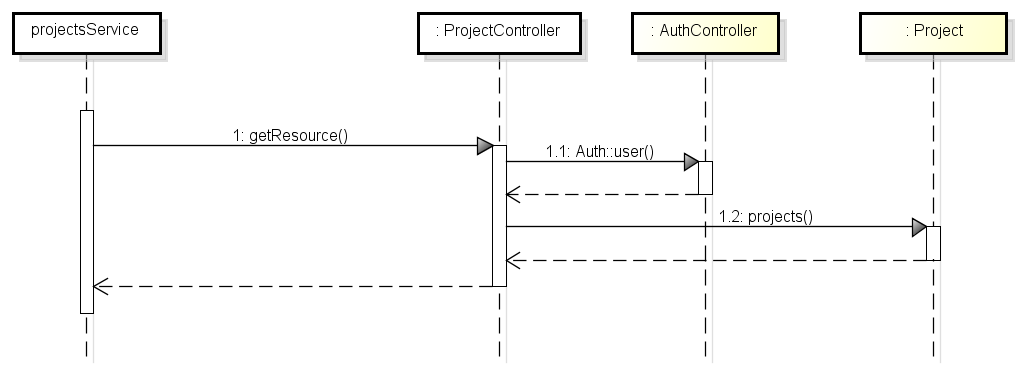
\includegraphics[width=0.7\linewidth]{img/GET_projects}
	\caption[GET user/:username/project]{GET user/:username/project}
	\label{fig:GET user/:username/project}
\end{figure}

\paragraph{POST user/:username/project}
\begin{figure}[h]
	\centering
	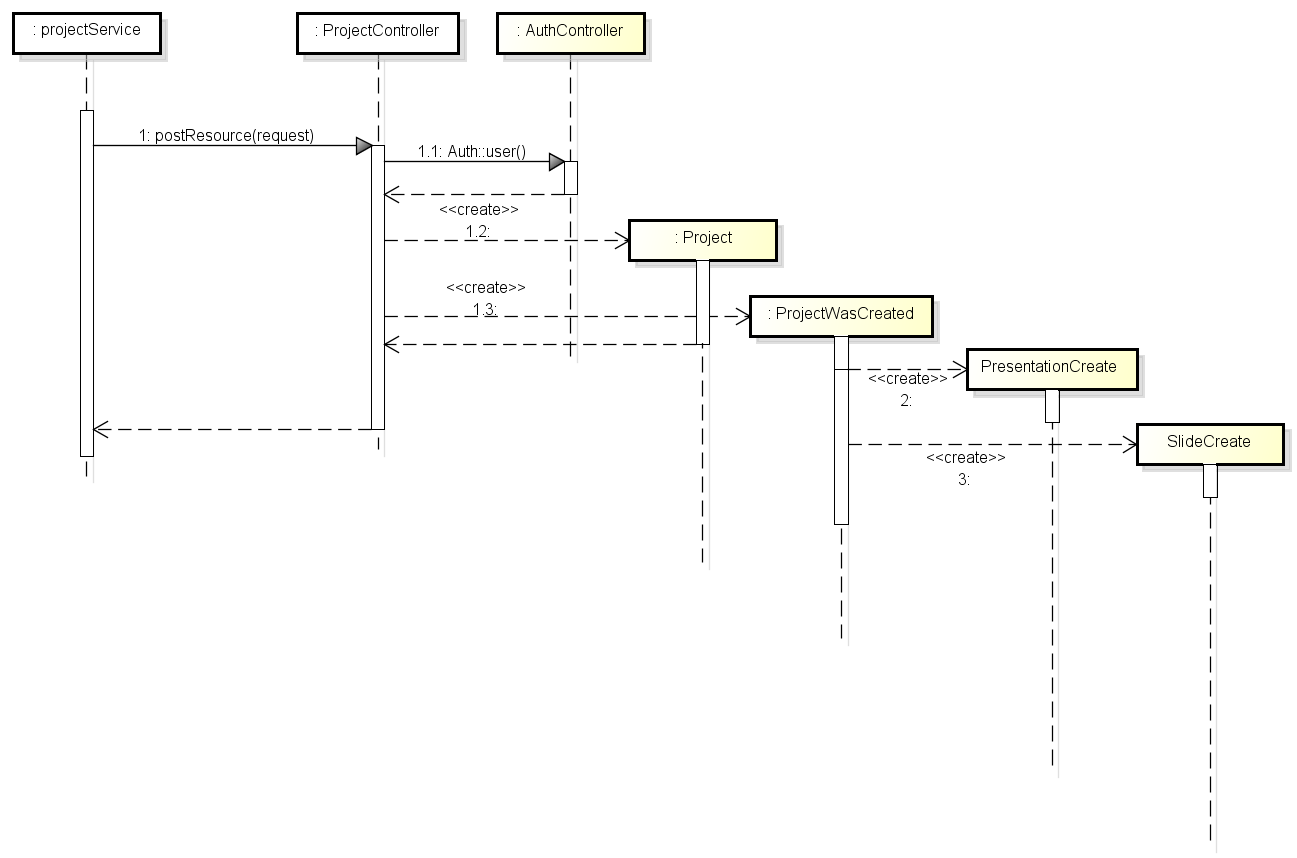
\includegraphics[width=0.7\linewidth]{img/POST_project}
	\caption[POST user/:username/project]{POST user/:username/project}
	\label{fig:POST user/:username/project}
\end{figure}

\newpage

\paragraph{PUT user/:username/project/:projectID}
\begin{figure}[h]
	\centering
	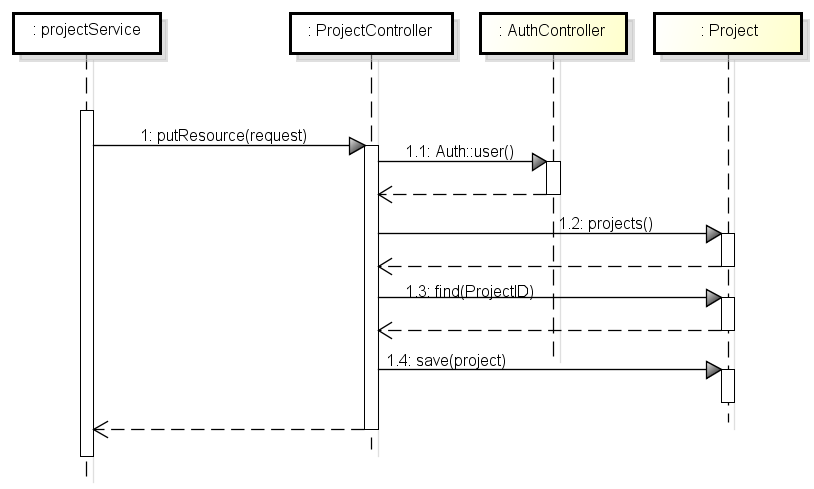
\includegraphics[width=0.7\linewidth]{img/PUT_project}
	\caption[PUT user/:username/project/:projectID]{PUT user/:username/project/:projectID}
	\label{fig:PUT user/:username/project/projectID}
\end{figure}

\paragraph{DELETE user/:username/project/projectID}
\begin{figure}[h]
	\centering
	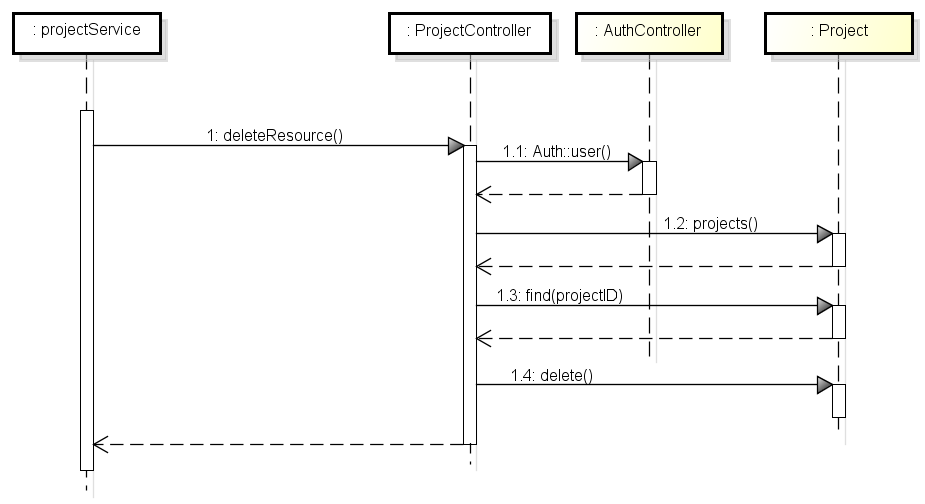
\includegraphics[width=0.7\linewidth]{img/DELETE_project}
	\caption[DELETE user/:username/project/:projectID]{DELETE user/:username/project/:projectID}
	\label{fig:DELETE user/:username/project/:projectID}
\end{figure}
\newpage

\newpage

\section{Tracciamento}
\subsection{Tracciamento test-metodi}
\begin{table}[h]
	\begin{center}
	\begin{tabular}{|l|p{0.3\textwidth}|p{0.4\textwidth}|c|}
	\toprule
		\textbf{Test}  & \textbf{Metodi}\\
		
	\midrule
		TU1 & ChartCtrl :: load() , ChartCtrl :: save() \\
	\midrule
		TU2 & ImageCtrl :: upload() ,ImageCtrl :: load() , ImageCtrl :: save() \\
	\midrule
		TU3 & RealTimeDataCtrl :: load() , RealTimeDataCtrl :: save() \\
	\midrule
		TU4 & TableCtrl :: load() \\
	\midrule
		TU5 &TextCtrl :: load() \\
	\midrule
		TU6 &InfographicEditorCtrl :: addElement() \\
	\midrule
		TU7 & AuthenticationCtrl :: register(username:String,password:String) , AuthenticationCtrl :: logIn() , AuthenticationCtrl :: logOut() \\
\bottomrule
\end{tabular}
\end{center}
\end{table}

\begin{table}[H]
\begin{center}
\begin{tabular}{|l|p{0.3\textwidth}|p{0.4\textwidth}|c|}

	\toprule
		TU8 & AuthenticationCtrl :: registerViaFacebook(name:Boolean) , AuthenticationCtrl :: registerViaGooglePlus(query:Boolean) \\
	\midrule
		TU9 & AuthenticationCtrl :: forgotPassword(username:String) \\
	\midrule
		TU10 & PresentationEditorCtrl :: addSlide(direction: String) \\
	\midrule
		TU11 & PresentationEditorCtrl :: removeSlide() \\
	\midrule
		TU12 & PresentationEditorCtrl :: loadSlide(direction: String) \\
	\midrule
		TU13 & PresentationEditorCtrl :: saveSlide() \\
	\midrule
		TU14 & ProjectCtrl :: resetPresentation() \\
	\midrule
		TU15 & ProjectCtrl :: addInfographic() , ProjectCtrl :: deleteInfographic(id:Int) \\
			\bottomrule
\end{tabular}
\end{center}
\end{table}
\begin{table}[H]
\begin{center}
\begin{tabular}{|l|p{0.3\textwidth}|p{0.4\textwidth}|c|}

	\toprule
		TU16 & SlideEditorCtrl :: addObject():Int \\
	\midrule
		TU17 & SlideEditorCtrl :: removeObject(id:String) \\
	\midrule
		TU18 & SlideEditorCtrl :: udpateObject(id:String) \\

	\midrule
		TU19 & MyAccountCtrl :: loadUserdata(userId:String) \\
	\midrule
		TU20 & HomePageCtrl :: searchByUsername(text:String) \\
	\midrule
		TU21 & HomePageCtrl :: searchByProjectName(text:String) \\
	\midrule
		TU22 & InfographicEditorCtrl :: addElement(position:Int, id:Int) \\
	\midrule
		TU23 & InfographicEditorCtrl :: removeElement(position:Int) \\
	\midrule
			TU24 & InfographicEditorCtrl :: setTemplate(Tid:Int) \\
			\midrule
			TU25 & InfographicEditorCtrl :: getSlideList() \\
			\midrule
			TU26 & forgotPasswordService ::  save(data: Object) , loginService :: save(data: Object) , logoutService :: get() , signUpService :: save(data: Object) , userService :: query(id:String) \\
			\midrule
			TU27 & infographicEditorService :: query(id: String) , infographicEditorService :: save(name: String) , infographicEditorService :: update(id: String, data:Object) \\
			\midrule
			TU28 & presentationService :: query(id: String) , presentationService :: update(id: String, theme:String, transition:String) \\

\bottomrule

\end{tabular}
\end{center}
\end{table}
\begin{table}[H]
\begin{center}
\begin{tabular}{|l|p{0.3\textwidth}|p{0.4\textwidth}|c|}

	\toprule
	

		TU29 & projectsService :: query(username: String) , projectsService :: save(id: String, data:Object) \\
	\midrule
		TU30 & searchByProjectService ::  query(name: String) \\
	\midrule
		TU31 & projectService :: delete(id: String) , projectService :: update(id: String, data:Object) \\
	\midrule
		TU32 & indexService :: get(id: String, xIndex:int, yIndex:int) , slideService :: get(id:String) , slideService :: save(xIndex:int, yIndex:int) , slideService :: update(id:String, xIndex:int, yIndex:int, components:JSON, background:String,
slideSVG:SVG) , slideService :: delete(id:String) \\

	\bottomrule
	\end{tabular}
	\end{center}
	\caption{Tabella di tracciamento test-metodi}
\end{table}
\newpage
\subsection{Tracciamento requisiti-classi}
\begin{table}[h]
	\begin{center}
		\begin{tabular}{|p{0.2\linewidth}|p{0.75\linewidth}|}
			\toprule
			\textbf{Requisiti} & \textbf{Classe}\\
		\midrule
			R[OBB][F]1 & Premi::Http::Controllers::Auth::AuthController , Premi::Front-End::Controllers::AuthenticationCtrl , Premi::Front-End::Services::AuthenticationService , Premi::Front-End::Views::Signup\\
		\midrule
			R[OBB][F]1.1 & Premi::Http::Controllers::Auth::AuthController , Premi::Front-End::Controllers::AuthenticationCtrl\\
		\midrule
			R[OBB][F]1.1.1 & Premi::Http::Controllers::Auth::AuthController\\
		\midrule
			R[OBB][F]1.1.2 & Premi::Http::Controllers::Auth::AuthController\\
		\midrule
			R[OBB][F]1.2 & Premi::Http::Controllers::Auth::AuthController , Premi::Front-End::Controllers::AuthenticationCtrl\\
		\midrule
			R[OBB][F]1.2.1 & Premi::Http::Controllers::Auth::AuthController\\
		\midrule
			R[OBB][F]1.2.2 & Premi::Http::Controllers::Auth::AuthController\\
		\midrule
			R[OBB][F]1.3 & Premi::Http::Controllers::Auth::AuthController , Premi::Front-End::Controllers::AuthenticationCtrl\\
		\midrule
			R[OBB][F]1.3.1 & Premi::Http::Controllers::Auth::AuthController\\
		\midrule
			R[OBB][F]1.4 & Premi::Http::Controllers::Auth::AuthController , Premi::Front-End::Controllers::AuthenticationCtrl\\
		\midrule
			R[OBB][F]1.4.1 & Premi::Http::Controllers::Auth::AuthController\\
		\midrule
			R[OBB][F]1.5 & Premi::Http::Controllers::Auth::AuthController , Premi::Front-End::Controllers::AuthenticationCtrl\\
		\midrule
			R[OBB][F]1.5.1 & Premi::Http::Controllers::Auth::AuthController\\
		\midrule
			R[OPZ][F]1.6 & -\\
		\midrule
			R[OPZ][F]1.6.1 & -\\
		\midrule
			R[OPZ][F]1.6.2 & -\\
		\midrule
			R[OPZ][F]1.6.3 & -\\
		\midrule
			R[OPZ][F]1.6.1.1 & -\\
		\midrule
			R[OPZ][F]1.6.2.1 & -\\
		\midrule
			R[OPZ][F]1.6.3.1 & -\\
		\midrule
			R[OPZ][F]1.6.4 & Premi::Http::Controllers::Auth::AuthController , Premi::Front-End::Controllers::AuthenticationCtrl\\
		\midrule
			R[OBB][F]1.7 & Premi::Http::Controllers::Auth::AuthController , Premi::Front-End::Controllers::AuthenticationCtrl\\
		
		\bottomrule
	\end{tabular}
\end{center}
\end{table}


\begin{table}[h]
	\begin{center}
		\begin{tabular}{|p{0.2\linewidth}|p{0.75\linewidth}|}
			\toprule
			R[OBB][F]1.7.1 & Premi::Http::Controllers::Auth::AuthController , Premi::Front-End::Controllers::AuthenticationCtrl\\
		\midrule
			R[OBB][F]1.7.2 & Premi::Http::Controllers::Auth::AuthController , Premi::Front-End::Controllers::AuthenticationCtrl\\
		\midrule
			R[OBB][F]2 & Premi::Http::Controllers::Auth::AuthController , Premi::Front-End::Controllers::AuthenticationCtrl , Premi::Front-End::Services::AuthenticationService , Premi::Front-End::Views::Login\\
		\midrule
			R[OBB][F]2.1 & Premi::Http::Controllers::Auth::AuthController , Premi::Front-End::Controllers::AuthenticationCtrl\\
		\midrule
			R[OBB][F]2.2 & Premi::Http::Controllers::Auth::AuthController , Premi::Front-End::Controllers::AuthenticationCtrl\\
		\midrule
			R[OBB][F]2.3 & Premi::Http::Controllers::Auth::AuthController , Premi::Front-End::Controllers::AuthenticationCtrl\\
		\midrule
			R[OBB][F]2.4 & Premi::Http::Controllers::Auth::AuthController , Premi::Front-End::Controllers::AuthenticationCtrl\\
		\midrule
			R[OBB][F]2.5 & Premi::Http::Controllers::Auth::PasswordController , Premi::Front-End::Controllers::AuthenticationCtrl\\
		\midrule
			R[OBB][F]2.5.1 & Premi::Http::Controllers::Auth::PasswordController , Premi::Front-End::Controllers::AuthenticationCtrl\\
		\midrule
			R[OBB][F]3 & Premi::Http::Controllers::ProjectController , Premi::Front-End::Controllers::HomePageCtrl , Premi::Front-End::Services::SearchService , Premi::Front-End::Views::Search\\
		\midrule
			R[OBB][F]3.1 & Premi::Http::Controllers::ProjectController , Premi::Front-End::Controllers::HomePageCtrl\\
		\midrule
			R[OBB][F]3.2 & Premi::Http::Controllers::ProjectController , Premi::Front-End::Controllers::HomePageCtrl\\
		\midrule
			R[OBB][F]3.3 & Premi::Http::Controllers::ProjectController , Premi::Front-End::Controllers::HomePageCtrl\\
		\midrule
			R[OBB][F]3.4 & Premi::Http::Controllers::ProjectController , Premi::Front-End::Controllers::HomePageCtrl\\
		\midrule
			R[OBB][F]3.5 & Premi::Http::Controllers::ProjectController , Premi::Front-End::Controllers::HomePageCtrl\\
		\midrule
			R[OBB][F]4 & Premi::Http::Controllers::ProjectController , Premi::Front-End::Controllers::PresentationCtrl , Premi::Front-End::Services::PresentationService , Premi::Front-End::Views::Presentation\\
		\midrule
			R[OBB][F]4.1 & Premi::Http::Controllers::PresentationController , Premi::Front-End::Controllers::PresentationCtrl\\
		\midrule
			R[OBB][F]4.1.1 & Premi::Http::Controllers::PresentationController , Premi::Front-End::Controllers::PresentationCtrl\\

\bottomrule
\end{tabular}
\end{center}
\end{table}


\begin{table}[h]
	\begin{center}
		\begin{tabular}{|p{0.2\linewidth}|p{0.75\linewidth}|}
			\toprule
			R[OBB][F]4.1.1.1 & Premi::Http::Controllers::SlideController , Premi::Front-End::Controllers::PresentationCtrl\\
		\midrule
			R[OBB][F]4.1.1.2 & Premi::Http::Controllers::SlideController , Premi::Front-End::Controllers::PresentationCtrl\\
		\midrule
			R[OBB][F]4.1.1.3 & -\\
		\midrule
			R[OBB][F]4.1.1.4 & -\\
		\midrule
			R[OBB][F]4.1.2 & -\\
		\midrule
			R[OBB][F]4.1.2.1 & -\\
		\midrule
			R[OBB][F]4.1.3 & -\\
		\midrule
			R[OPZ][F]4.2 & Premi::Http::Controllers::InfographicController , Premi::Front-End::Controllers::InfographicEditorCtrl\\
		\midrule
			R[OBB][F]5  & -\\
		\midrule
			R[OBB][F]5.1 & -\\
		\midrule
			R[OBB][F]5.2 & -\\
		\midrule
			R[OBB][F]6 & -\\
		\midrule
			R[OBB][F]6.1 & -\\
		\midrule
			R[OBB][F]7 & Premi::Http::Controllers::ProjectController , Premi::Front-End::Controllers::ProjectsCtrl , Premi::Front-End::Services::ProjectService , Premi::Front-End::Views::Projects\\
		\midrule
			R[OBB][F]7.1 & Premi::Model::Project , Premi::Front-End::Controllers::ProjectsCtrl\\
		\midrule
			R[OBB][F]7.2 & Premi::Http::Controllers::ProjectController , Premi::Front-End::Controllers::PresentationEditorCtrl\\
		\midrule
			R[OBB][F]8 & Premi::Http::Controllers::ProjectController , Premi::Front-End::Controllers::ProjectsCtrl , Premi::Front-End::Services::ProjectService , Premi::Front-End::Views::Projects\\
		\midrule
			R[OBB][F]9 & Premi::Http::Controllers::SlideController , Premi::Front-End::Controllers::SlideEditorCtrl , Premi::Front-End::Controllers:PresentationCtrl , Premi::Front-End::Services::SlideService  , Premi::Front-End::Views::PresentationEditor , Premi::Front-End::Views::SlideEditor\\
		\bottomrule
		\end{tabular}
	\end{center}
\end{table}
	

\begin{table}[h]
	\begin{center}
		\begin{tabular}{|p{0.2\linewidth}|p{0.75\linewidth}|}
			\toprule
			R[OBB][F]9.1 & Premi::Http::Controllers::SlideController , Premi::Front-End::Controllers::PresentationEditorCtrl\\
		\midrule
			R[OBB][F]9.2 & Premi::Http::Controllers::SlideController , Premi::Front-End::Controllers::PresentationEditorCtrl\\
		\midrule
			R[OBB][F]9.2.1 & Premi::Http::Controllers::SlideController , Premi::Front-End::Controllers::PresentationEditorCtrl\\
		\midrule
			R[OBB][F]9.2.2 & Premi::Http::Controllers::SlideController , Premi::Front-End::Controllers::PresentationEditorCtrl\\
		\midrule
			R[OBB][F]9.3 & Premi::Http::Controllers::SlideController , Premi::Front-End::Controllers::PresentationEditorCtrl\\
		\midrule
			R[OBB][F]9.4 & Premi::Model::Image , Premi::Front-End::Controllers::SlideEditorCtrl , Premi::Front-End::Views::Component\\
		\midrule
			R[OBB][F]9.4.1 & Premi::Model::Image\\
		\midrule
			R[OBB][F]9.4.2 & Premi::Model::Image\\
		\midrule
			R[OBB][F]9.4.3 & Premi::Model::Image\\
		\midrule
			R[OBB][F]9.5 & Premi::Model::Text , Premi::Front-End::Controllers::SlideEditorCtrl , Premi::Front-End::Views::Component\\
		\midrule
			R[OPZ][F]9.6 & Premi::Model::RealTimeData , Premi::Front-End::Controllers::SlideEditorCtrl\\
		\midrule
			R[OPZ][F]9.6.1 & Premi::Model::Image , Premi::Front-End::Controllers::SlideEditorCtrl\\
		\midrule
			R[OPZ][F]9.6.2 & -\\
		\midrule
			R[OPZ][F]9.6.3 & -\\
		\midrule
			R[OPZ][F]9.6.4 & -\\
		\midrule
			R[OPZ][F]9.6.5 & -\\
		\midrule
			R[OBB][F]9.7 & Premi::Model::Tabel\\
		\midrule
			R[OBB][F]9.7.1 & Premi::Model::Table\\
		\midrule
			R[OBB][F]9.7.2 & Premi::Model::Table\\
		\midrule
			R[OPZ][F]9.8 & Premi::Model::Chart\\
		\midrule
			R[OPZ][F]9.8.1 & Premi::Model::Chart\\
		\midrule
			R[OPZ][F]9.8.1.1 & Premi::Model::Chart\\
		\midrule
			R[OPZ][F]9.8.1.2 & Premi::Model::Chart\\
		\midrule
			R[OPZ][F]9.8.1.3 & Premi::Model::Chart\\
		\midrule
			R[OPZ][F]9.8.2 & Premi::Model::Chart\\
		\midrule
			R[OPZ][F]9.8.3 & Premi::Model::Chart\\
		\midrule
			R[OPZ][F]9.8.4 & Premi::Model::Chart\\
		\bottomrule
		\end{tabular}
	\end{center}
\end{table}

\begin{table}[h]
	\begin{center}
		\begin{tabular}{|p{0.2\linewidth}|p{0.75\linewidth}|}
			\toprule
			R[OBB][F]9.9 & Premi::Model::Presentation , Premi::Front-End::Controllers::PresentationEditorCtrl\\
		\midrule
			R[OBB][F]9.9.1 & Premi::Model::Presentation , Premi::Front-End::Controllers::PresentationEditorCtrl\\
		\midrule
			R[OBB][F]9.9.2 & Premi::Model::Presentation , Premi::Front-End::Controllers::PresentationEditorCtrl\\
		\midrule
			R[OBB][F]9.9.3 & Premi::Model::Presentation , Premi::Front-End::Controllers::PresentationEditorCtrl\\
		\midrule
			R[OBB][F]9.9.4 & Premi::Model::Presentation , Premi::Front-End::Controllers::PresentationEditorCtrl\\
		\midrule
			R[OBB][F]9.9.5 & Premi::Model::Presentation , Premi::Front-End::Controllers::PresentationEditorCtrl\\
		\midrule
			R[OBB][F]9.10 & Premi::Front-End::Controllers::SlideEditorCtrl\\
		\midrule
			R[OBB][F]9.11 & Premi::Front-End::Controllers::SlideEditorCtrl\\
		\midrule
			R[OBB][F]9.12 & Premi::Front-End::Controllers::SlideEditorCtrl\\
		\midrule
			R[OBB][F]9.13 & Premi::Front-End::Controllers::SlideEditorCtrl\\
		\midrule
			R[OBB][F]9.14 & -\\
		\midrule
			R[OBB][F]9.15 & Premi::Front-End::Controllers::SlideEditorCtrl\\
		\midrule
			R[OBB][F]9.15.1 & Premi::Front-End::Controllers::SlideEditorCtrl\\
		\midrule
			R[OBB][F]9.15.2 & Premi::Front-End::Controllers::SlideEditorCtrl\\
		\midrule
			R[OBB][F]9.15.3 & Premi::Front-End::Controllers::SlideEditorCtrl\\
		\midrule
			R[OBB][F]9.15.4 & Premi::Front-End::Controllers::SlideEditorCtrl\\
		\midrule
			R[OBB][F]9.15.5 & Premi::Front-End::Controllers::SlideEditorCtrl\\
		\midrule
			R[OBB][F]9.15.6 & Premi::Front-End::Controllers::SlideEditorCtrl\\
		\midrule
			R[OBB][F]9.15.7 & Premi::Front-End::Controllers::SlideEditorCtrl\\
		\midrule
			R[OBB][F]9.16 & -\\
		\midrule
			R[OBB][F]9.16.1 & -\\
		\midrule
			R[OBB][F]9.16.2 & -\\
		\midrule
			R[OBB][F]9.16.3 & -\\
		\midrule
			R[OBB][F]9.16.4 & -\\
		\midrule
			R[OBB][F]9.16.5 & -\\
		\midrule
			R[OBB][F]9.16.6 & -\\
		\midrule
			R[OPZ][F]9.17 & -\\
		\midrule
			R[OPZ][F]9.17.1 & -\\
		\midrule
			R[OPZ][F]9.17.2 & -\\
		\midrule
			R[OPZ][F]9.17.3 & -\\
		\midrule
			R[OPZ][F]9.17.4 & -\\
		\midrule
			R[OPZ][F]9.17.5 & -\\
		\bottomrule
		\end{tabular}
	\end{center}
\end{table}


\begin{table}[h]
	\begin{center}
		\begin{tabular}{|p{0.2\linewidth}|p{0.75\linewidth}|}
			\toprule
			R[OPZ][F]9.17.5.1 & -\\
		\midrule
			R[OPZ][F]9.17.5.2 & -\\
		\midrule
			R[OPZ][F]9.17.5.3 & -\\
		\midrule
			R[OPZ][F]9.17.6 & -\\
		\midrule
			R[OPZ][F]9.17.7 & -\\
		\midrule
			R[OPZ][F]9.18 & -\\
		\midrule
			R[OPZ][F]9.19 & -\\
		\midrule
			R[DES][F]10 & Premi::Model::Infographic , Premi::Front-End::Views::InfographicEditor , Premi::Front-End::Services::InfographicService\\
		\midrule
			R[DES][F]10.1 & -\\
		\midrule
			R[DES][F]10.2 & -\\
		\midrule
			R[OBB][F]11 & Premi::Http::Controllers::ProjectController , Premi::Front-End::Controllers::PresentationCtrl , Premi::Front-End::Services::PresentationService , Premi::Front-End::Views::PresentationEditor\\
		\midrule
			R[OBB][F]11.1 & -\\
		\midrule
			R[OBB][F]11.2 & -\\
		\midrule
			R[OBB][F]12 & Premi::Http::Controllers::ProjectController , Premi::Front-End::Controllers::ProjectCtrl , Premi::Front-End::Services::PresentationService , Premi::Front-End::Views::Project\\
		\midrule
			R[OBB][F]12.1 & Premi::Front-End::Controllers::PresentationCtrl\\
		\midrule
			R[OBB][F]12.2.1 & Premi::Front-End::Controllers::PresentationCtrl\\
		\midrule
			R[OBB][F]12.2.2 & Premi::Front-End::Controllers::PresentationCtrl\\
		\midrule
			R[OBB][F]13 & -\\
			\bottomrule
		\end{tabular}
	\end{center}
	\caption{Tabella di tracciamento requisiti-classe}
\end{table}
\newpage
\newpage
\begin{table}[h]
	\caption{Tabella di tracciamento classi-requisiti}
	\begin{center}
		\begin{tabular}{|p{0.75\linewidth}|p{0.2\linewidth}|}
			\toprule
			\textbf{Requisiti} & \textbf{Classe}\\
		\midrule
			 Premi::Http::Controllers::Auth::AuthController , Premi::Front-End::Controllers::AuthenticationCtrl , Premi::Front-End::Services::AuthenticationService , Premi::Front-End::Views::Signup & R[OBB][F]1 \\
		\midrule
			 Premi::Http::Controllers::Auth::AuthController , Premi::Front-End::Controllers::AuthenticationCtrl & R[OBB][F]1.1 \\
		\midrule
			Premi::Http::Controllers::Auth::AuthController & R[OBB][F]1.1.1 \\
		\midrule
			Premi::Http::Controllers::Auth::AuthController & R[OBB][F]1.1.2 \\
		\midrule
            Premi::Http::Controllers::Auth::AuthController , Premi::Front-End::Controllers::AuthenticationCtrl & R[OBB][F]1.2 \\
		\midrule
			Premi::Http::Controllers::Auth::AuthController & R[OBB][F]1.2.1 \\
		\midrule
		  Premi::Http::Controllers::Auth::AuthController & R[OBB][F]1.2.2 \\
		\midrule
		  Premi::Http::Controllers::Auth::AuthController , Premi::Front-End::Controllers::AuthenticationCtrl & R[OBB][F]1.3 \\
		\midrule
			Premi::Http::Controllers::Auth::AuthController & R[OBB][F]1.3.1 \\
		\midrule
			Premi::Http::Controllers::Auth::AuthController , Premi::Front-End::Controllers::AuthenticationCtrl & R[OBB][F]1.4 \\
		\midrule
			Premi::Http::Controllers::Auth::AuthController & R[OBB][F]1.4.1 \\
		\midrule
			Premi::Http::Controllers::Auth::AuthController , Premi::Front-End::Controllers::AuthenticationCtrl & R[OBB][F]1.5 \\
		\midrule
			Premi::Http::Controllers::Auth::AuthController & R[OBB][F]1.5.1 \\
		\midrule
			 & R[OPZ][F]1.6 \\
		\midrule
			- & R[OPZ][F]1.6.1 \\
		\midrule
			- & R[OPZ][F]1.6.2 \\
		\midrule
			- & R[OPZ][F]1.6.3 \\
		\midrule
			- & R[OPZ][F]1.6.1.1 \\
		\midrule
			- & R[OPZ][F]1.6.2.1 \\
		\midrule
			- & R[OPZ][F]1.6.3.1 \\
		\midrule
			Premi::Http::Controllers::Auth::AuthController , Premi::Front-End::Controllers::AuthenticationCtrl & R[OPZ][F]1.6.4 \\
		\midrule
			Premi::Http::Controllers::Auth::AuthController , Premi::Front-End::Controllers::AuthenticationCtrl & R[OBB][F]1.7 \\
		
		\bottomrule
	\end{tabular}
\end{center}
\end{table}


\begin{table}[h]
	\begin{center}
		\begin{tabular}{|p{0.75\linewidth}|p{0.2\linewidth}|}
			\toprule
			Premi::Http::Controllers::Auth::AuthController , Premi::Front-End::Controllers::AuthenticationCtrl & R[OBB][F]1.7.1 \\
		\midrule
			Premi::Http::Controllers::Auth::AuthController , Premi::Front-End::Controllers::AuthenticationCtrl & R[OBB][F]1.7.2 \\
		\midrule
			Premi::Http::Controllers::Auth::AuthController , Premi::Front-End::Controllers::AuthenticationCtrl , Premi::Front-End::Services::AuthenticationService , Premi::Front-End::Views::Login & R[OBB][F]2 \\
		\midrule
			Premi::Http::Controllers::Auth::AuthController , Premi::Front-End::Controllers::AuthenticationCtrl & R[OBB][F]2.1 \\
		\midrule
			Premi::Http::Controllers::Auth::AuthController , Premi::Front-End::Controllers::AuthenticationCtrl & R[OBB][F]2.2 \\
		\midrule
			Premi::Http::Controllers::Auth::AuthController , Premi::Front-End::Controllers::AuthenticationCtrl & R[OBB][F]2.3 \\
		\midrule
			Premi::Http::Controllers::Auth::AuthController , Premi::Front-End::Controllers::AuthenticationCtrl & R[OBB][F]2.4 \\
		\midrule
			Premi::Http::Controllers::Auth::PasswordController , Premi::Front-End::Controllers::AuthenticationCtrl & R[OBB][F]2.5 \\
		\midrule
			Premi::Http::Controllers::Auth::PasswordController , Premi::Front-End::Controllers::AuthenticationCtrl & R[OBB][F]2.5.1 \\
		\midrule
			Premi::Http::Controllers::ProjectController , Premi::Front-End::Controllers::HomePageCtrl , Premi::Front-End::Services::SearchService , Premi::Front-End::Views::Search & R[OBB][F]3 \\
		\midrule
			Premi::Http::Controllers::ProjectController , Premi::Front-End::Controllers::HomePageCtrl & R[OBB][F]3.1 \\
		\midrule
			Premi::Http::Controllers::ProjectController , Premi::Front-End::Controllers::HomePageCtrl & R[OBB][F]3.2 \\
		\midrule
			Premi::Http::Controllers::ProjectController , Premi::Front-End::Controllers::HomePageCtrl & R[OBB][F]3.3 \\
		\midrule
			Premi::Http::Controllers::ProjectController , Premi::Front-End::Controllers::HomePageCtrl & R[OBB][F]3.4 \\
		\midrule
			Premi::Http::Controllers::ProjectController , Premi::Front-End::Controllers::HomePageCtrl & R[OBB][F]3.5 \\
		\midrule
			Premi::Http::Controllers::ProjectController , Premi::Front-End::Controllers::PresentationCtrl , Premi::Front-End::Services::PresentationService , Premi::Front-End::Views::Presentation & R[OBB][F]4 \\
		\midrule
			Premi::Http::Controllers::PresentationController , Premi::Front-End::Controllers::PresentationCtrl & R[OBB][F]4.1 \\
		\midrule
			Premi::Http::Controllers::PresentationController , Premi::Front-End::Controllers::PresentationCtrl & R[OBB][F]4.1.1 \\

\bottomrule
\end{tabular}
\end{center}
\end{table}


\begin{table}[h]
	\begin{center}
		\begin{tabular}{|p{0.75\linewidth}|p{0.2\linewidth}|}
			\toprule
			Premi::Http::Controllers::SlideController , Premi::Front-End::Controllers::PresentationCtrl & R[OBB][F]4.1.1.1 \\
		\midrule
			Premi::Http::Controllers::SlideController , Premi::Front-End::Controllers::PresentationCtrl & R[OBB][F]4.1.1.2 \\
		\midrule
			- & R[OPZ][F]4.1.1.3 \\
		\midrule
			Premi::Front-End::Controllers::PresentationCtrl & R[OBB][F]4.1.1.4 \\
		\midrule
			Premi::Http::Controllers::SlideController , Premi::Front-End::Controllers::PresentationCtrl & R[OBB][F]4.1.2 \\
		\midrule
			Premi::Http::Controllers::SlideController , Premi::Front-End::Controllers::PresentationCtrl & R[OBB][F]4.1.2.1 \\
		\midrule
			Premi::Http::Controllers::SlideController , Premi::Front-End::Controllers::PresentationCtrl & R[OBB][F]4.1.3 \\
		\midrule
			Premi::Http::Controllers::InfographicController , Premi::Front-End::Controllers::InfographicEditorCtrl & R[OPZ][F]4.2 \\
		\midrule
			Premi::Front-End::Controllers::PresentationCtrl & R[OBB][F]5  \\
		\midrule
			Premi::Front-End::Controllers::PresentationCtrl & R[OBB][F]5.1 \\
		\midrule
			Premi::Front-End::Controllers::PresentationCtrl & R[OBB][F]5.2 \\
		\midrule
			Premi::Front-End::Controllers::ProjectCtrl & R[OBB][F]6 \\
		\midrule
			Premi::Front-End::Controllers::ProjectCtrl & R[OBB][F]6.1 \\
		\midrule
			Premi::Http::Controllers::ProjectController , Premi::Front-End::Controllers::ProjectsCtrl , Premi::Front-End::Services::ProjectService , Premi::Front-End::Views::Projects & R[OBB][F]7 \\
		\midrule
			Premi::Model::Project , Premi::Front-End::Controllers::ProjectsCtrl & R[OBB][F]7.1 \\
		\midrule
			Premi::Http::Controllers::ProjectController , Premi::Front-End::Controllers::PresentationEditorCtrl & R[OBB][F]7.2 \\
		\midrule
			Premi::Http::Controllers::ProjectController , Premi::Front-End::Controllers::ProjectsCtrl , Premi::Front-End::Services::ProjectService , Premi::Front-End::Views::Projects & R[OBB][F]8 \\
		\midrule
			Premi::Http::Controllers::SlideController , Premi::Front-End::Controllers::SlideEditorCtrl , Premi::Front-End::Controllers:PresentationCtrl , Premi::Front-End::Services::SlideService  , Premi::Front-End::Views::PresentationEditor , Premi::Front-End::Views::SlideEditor & R[OBB][F]9 \\
		\bottomrule
		\end{tabular}
	\end{center}
\end{table}
	

\begin{table}[h]
	\begin{center}
		\begin{tabular}{|p{0.75\linewidth}|p{0.2\linewidth}|}
			\toprule
			Premi::Http::Controllers::SlideController , Premi::Front-End::Controllers::PresentationEditorCtrl & R[OBB][F]9.1 \\
		\midrule
			Premi::Http::Controllers::SlideController , Premi::Front-End::Controllers::PresentationEditorCtrl & R[OBB][F]9.2 \\
		\midrule
			Premi::Http::Controllers::SlideController , Premi::Front-End::Controllers::PresentationEditorCtrl & R[OBB][F]9.2.1 \\
		\midrule
			Premi::Http::Controllers::SlideController , Premi::Front-End::Controllers::PresentationEditorCtrl & R[OBB][F]9.2.2 \\
		\midrule
			Premi::Http::Controllers::SlideController , Premi::Front-End::Controllers::PresentationEditorCtrl & R[OBB][F]9.3 \\
		\midrule
			Premi::Model::Image , Premi::Front-End::Controllers::SlideEditorCtrl , Premi::Front-End::Views::Component & R[OBB][F]9.4 \\
		\midrule
			Premi::Model::Image & R[OBB][F]9.4.1 \\
		\midrule
			Premi::Model::Image & R[OBB][F]9.4.2 \\
		\midrule
			Premi::Model::Image & R[OBB][F]9.4.3 \\
		\midrule
			Premi::Model::Text , Premi::Front-End::Controllers::SlideEditorCtrl , Premi::Front-End::Views::Component & R[OBB][F]9.5 \\
		\midrule
			Premi::Model::RealTimeData , Premi::Front-End::Controllers::SlideEditorCtrl & R[OPZ][F]9.6 \\
		\midrule
			Premi::Model::Image , Premi::Front-End::Controllers::SlideEditorCtrl & R[OPZ][F]9.6.1 \\
		\midrule
			- & R[OPZ][F]9.6.2 \\
		\midrule
			- & R[OPZ][F]9.6.3 \\
		\midrule
			- & R[OPZ][F]9.6.4 \\
		\midrule
			- & R[OPZ][F]9.6.5 \\
		\midrule
			Premi::Model::Tabel & R[OBB][F]9.7 \\
		\midrule
			Premi::Model::Table & R[OBB][F]9.7.1 \\
		\midrule
			Premi::Model::Table & R[OBB][F]9.7.2 \\
		\midrule
			Premi::Model::Chart & R[OPZ][F]9.8 \\
		\midrule
			Premi::Model::Chart & R[OPZ][F]9.8.1 \\
		\midrule
			Premi::Model::Chart & R[OPZ][F]9.8.1.1 \\
		\midrule
			Premi::Model::Chart & R[OPZ][F]9.8.1.2 \\
		\midrule
			Premi::Model::Chart & R[OPZ][F]9.8.1.3 \\
		\midrule
			Premi::Model::Chart & R[OPZ][F]9.8.2 \\
		\midrule
			Premi::Model::Chart & R[OPZ][F]9.8.3 \\
		\midrule
			Premi::Model::Chart & R[OPZ][F]9.8.4 \\
		\bottomrule
		\end{tabular}
	\end{center}
\end{table}

\begin{table}[h]
	\begin{center}
		\begin{tabular}{|p{0.75\linewidth}|p{0.2\linewidth}|}
			\toprule
			Premi::Model::Presentation , Premi::Front-End::Controllers::PresentationEditorCtrl & R[OBB][F]9.9 \\
		\midrule
			Premi::Model::Presentation , Premi::Front-End::Controllers::PresentationEditorCtrl & R[OBB][F]9.9.1 \\
		\midrule
			Premi::Model::Presentation , Premi::Front-End::Controllers::PresentationEditorCtrl & R[OBB][F]9.9.2 \\
		\midrule
			Premi::Model::Presentation , Premi::Front-End::Controllers::PresentationEditorCtrl & R[OBB][F]9.9.3 \\
		\midrule
			Premi::Model::Presentation , Premi::Front-End::Controllers::PresentationEditorCtrl & R[OBB][F]9.9.4 \\
		\midrule
			Premi::Model::Presentation , Premi::Front-End::Controllers::PresentationEditorCtrl & R[OBB][F]9.9.5 \\
		\midrule
			Premi::Front-End::Controllers::SlideEditorCtrl & R[OBB][F]9.10 \\
		\midrule
			Premi::Front-End::Controllers::SlideEditorCtrl & R[OBB][F]9.11 \\
		\midrule
			Premi::Front-End::Controllers::SlideEditorCtrl & R[OBB][F]9.12 \\
		\midrule
			Premi::Front-End::Controllers::SlideEditorCtrl & R[OBB][F]9.13 \\
		\midrule
			Premi::Front-End::Controllers::ImageCtrl & R[OBB][F]9.14 \\
		\midrule
			Premi::Front-End::Controllers::SlideEditorCtrl & R[OBB][F]9.15 \\
		\midrule
			Premi::Front-End::Controllers::SlideEditorCtrl & R[OBB][F]9.15.1 \\
		\midrule
			Premi::Front-End::Controllers::SlideEditorCtrl & R[OBB][F]9.15.2 \\
		\midrule
			Premi::Front-End::Controllers::SlideEditorCtrl & R[OBB][F]9.15.3 \\
		\midrule
			Premi::Front-End::Controllers::SlideEditorCtrl & R[OBB][F]9.15.4 \\
		\midrule
			Premi::Front-End::Controllers::SlideEditorCtrl & R[OBB][F]9.15.5 \\
		\midrule
			Premi::Front-End::Controllers::SlideEditorCtrl & R[OBB][F]9.15.6 \\
		\midrule
			Premi::Front-End::Controllers::SlideEditorCtrl & R[OBB][F]9.15.7 \\
		\midrule
			- & R[OPZ][F]9.16 \\
		\midrule
			- & R[OPZ][F]9.16.1 \\
		\midrule
			- & R[OPZ][F]9.16.2 \\
		\midrule
			- & R[OPZ][F]9.16.3 \\
		\midrule
			- & R[OPZ][F]9.16.4 \\
		\midrule
			- & R[OPZ][F]9.16.5 \\
		\midrule
			- & R[OPZ][F]9.16.6 \\
		\midrule
			- & R[OPZ][F]9.17 \\
		\midrule
			- & R[OPZ][F]9.17.1 \\
		\midrule
			- & R[OPZ][F]9.17.2 \\
		\midrule
			- & R[OPZ][F]9.17.3 \\
		\midrule
			- & R[OPZ][F]9.17.4 \\
		\midrule
			- & R[OPZ][F]9.17.5 \\
		\bottomrule
		\end{tabular}
	\end{center}
\end{table}


\begin{table}[h]
	\begin{center}
		\begin{tabular}{|p{0.75\linewidth}|p{0.2\linewidth}|}
			\toprule
			- & R[OPZ][F]9.17.5.1 \\
		\midrule
			- & R[OPZ][F]9.17.5.2 \\
		\midrule
			- & R[OPZ][F]9.17.5.3 \\
		\midrule
			- & R[OPZ][F]9.17.6 \\
		\midrule
			- & R[OPZ][F]9.17.7 \\
		\midrule
			- & R[OPZ][F]9.18 \\
		\midrule
			- & R[OPZ][F]9.19 \\
		\midrule
			Premi::Model::Infographic , Premi::Front-End::Views::InfographicEditor , Premi::Front-End::Services::InfographicService & R[DES][F]10 \\
		\midrule
			- & R[DES][F]10.1 \\
		\midrule
			- & R[DES][F]10.2 \\
		\midrule
			Premi::Http::Controllers::ProjectController , Premi::Front-End::Controllers::PresentationCtrl , Premi::Front-End::Services::PresentationService , Premi::Front-End::Views::PresentationEditor & R[OBB][F]11 \\
		\midrule
			- & R[OBB][F]11.1 \\
		\midrule
			- & R[OBB][F]11.2 \\
		\midrule
			Premi::Http::Controllers::ProjectController , Premi::Front-End::Controllers::ProjectCtrl , Premi::Front-End::Services::PresentationService , Premi::Front-End::Views::Project & R[OBB][F]12 \\
		\midrule
			Premi::Front-End::Controllers::PresentationCtrl & R[OBB][F]12.1 \\
		\midrule
			Premi::Front-End::Controllers::PresentationCtrl & R[OBB][F]12.2.1 \\
		\midrule
			Premi::Front-End::Controllers::PresentationCtrl & R[OBB][F]12.2.2 \\
		\midrule
			Premi::Front-End::View::PresentationEditor & R[OBB][F]13 \\
			\bottomrule
		\end{tabular}
	\end{center}
\end{table}
\newpage



%\printglossaries

\end{document}
